Las ondas gravitatorias las podemos dividir según su origen en dos tipos: astrofísicas y cosmológicas. Las ondas gravitatorias astrofísicas son aquellas que se producen como consecuencia de fenómenos astrofísicos tal como la unión de agujeros negros, las producidas al tener sistema binarios, las producidas por supernovas o púlsares. Por otro lado, tenemos las ondas gravitatorias cosmológicas que se producen por efectos cosmológicos tal como el Big Bang o distintos eventos históricos cosmológicos (entre los cuales entra el recalentamiento, alguna ruptura instantánea de simetría o alguna transición de fase), a las del primer tipo las llamaremos primordiales, mientras que las otras no tienen un nombre particular.

Otra distinción que se puede hacer a la hora de hablar de ondas gravitatorias es entre ondas coherentes e incoherentes. Las ondas coherentes son aquellas que cuando las medimos, podemos identificar cuál es su fuente; en cambio, las ondas incoherente son aquellas que forman un fondo estocástico, ésto implica que se pueden medir viendo correlaciones entre los sensores, pero al tener la medición no podemos identificar o clasificar las ondas que se dan por un fenómeno en particular.

Es importante tener en cuenta que los fenómenos cosmológicos sólo forman ondas incoherentes, mientras que los fenómenos astrofísicos pueden formar tanto ondas coherentes como incoherentes. Ésto genera una dificultad extra a la hora de querer identificar ondas de origen puramente cosmológico.

\subsection{Vacío de Bunch-Davies y la cuantización de las ondas en inflación}

A partir de la acción

\begin{equation*}
    \begin{split} 
        S^{(2)}_g &= - \frac{m_P^2}{8} \int a^2 (\eta) \ \eta^{\mu \nu} \partial_\mu h_{ij} \partial_\nu h_{ij} \ d^3 x \ d\eta\\
        &= \frac{m^2_P}{4 (2 \pi)^3} \int a^2 (\eta) \left[ \left| h'_r (\textbf{k}, \eta) \right| - k^2 h_r (\textbf{k}, \eta) \right] \ d^3 k \ d \eta\\
        &= \frac{1}{2 (2 \pi)^3} \sum_{r = +, \times} \int \left[ \left| v'_r (\textbf{k}, \eta) \right|^2 + \left( \frac{a^{\prime \prime}}{a} - k^2 \right) \left| v_r (\textbf{k}, \eta) \right|^2 \right] 
    \end{split}
\end{equation*}

\noindent
dónde $\displaystyle v_r = \frac{m_P}{\sqrt{2}} a h_r$. Podemos plantear un lagrangiano de la forma

\begin{equation}
    \mathcal{L} = \left( v^\prime_r \right)^2 + \left( \frac{a^{\prime \prime}}{a} - k^2 \right) v^2_r
\end{equation}

\noindent
ahora usemos las ecuaciones de Euler-Lagrange

\begin{equation}
    \frac{d}{d\eta} \left( \frac{\partial \mathcal{L}}{\partial v^\prime_r} \right) - \frac{\partial \mathcal{L}}{\partial v_r} = 0
\end{equation}

\begin{equation}\label{eqn:euler_lagrange_v}
    v^{\prime \prime}_r - \left( \frac{a^{\prime \prime}}{a} - k^2 \right) v_r = 0
\end{equation}

Esta es una ecuación de oscilador armónico de frecuencia $\displaystyle \omega^2 = k^2 - \frac{a^{\prime \prime}}{a}$, de modo tal que si esta frecuencia es negativa tendremos un antioscilador, mientras que si es positiva tendremos un oscilador. Se puede ver que para un universo de DeSitter $\displaystyle \frac{a^{\prime \prime}}{a} = \frac{2}{\eta^2}$ lo que implica que si $k \eta \ll 1$ (dentro del horizonte) la frecuencia será negativa y tendremos la amplificación de las perturbaciones y si $k \eta \gg 1$ (fuera del horizonte) tendremos frecuencia positiva y las perturbaciones no serán amplificadas. Esta ecuación, también nos permite escribir a los modos $v_r$ de forma de operador usando operadores de creación $\left( \hat{a}^\dagger \right)$ y de destrucción $\left( \hat{a} \right)$ como los osciladores armónicos

\begin{equation}\label{eqn:v_cuantizado}
    \hat{v}_r = \frac{1}{(2 \pi)^3} \int \left[ v_k \ e^{i k x} \ \hat{a}_{kr} + v_k^* \ e^{-ikx} \ \hat{a}_{kr}^\dagger \right] \ d^3 k
\end{equation}

\noindent
al cuantizar el campo debemos definir las condiciones de conmutación que en nuestro caso serán:

\begin{equation}
    \left[ \hat{v}_r \left( \textbf{x}, \eta \right), \hat{\pi}_{r'} \left( \textbf{x}', \eta \right) \right] = i \delta_{rr'} \delta \left( \textbf{x} - \textbf{x}' \right) \hspace{1cm} \left[ \hat{v}_r \left( \textbf{x}, \eta \right), \hat{v}_{r'} \left( \textbf{x}', \eta \right) \right] = \left[ \hat{\pi}_r \left( \textbf{x}, \eta \right), \hat{\pi}_{r'} \left( \textbf{x}', \eta \right) \right] = 0
\end{equation}

\begin{equation}
    \left[ \hat{a}_{kr}, \hat{a}^\dagger_{k'r'} \right] = (2 \pi)^3 \delta_{rr'} \delta \left( \textbf{k} - \textbf{k}' \right) \hspace{3cm} \left[ \hat{a}_{kr}, \hat{a}_{k'r'} \right] = \left[ \hat{a}^\dagger_{kr}, \hat{a}^\dagger_{k'r'} \right] = 0
\end{equation}

\noindent
dónde $\hat{\pi} = \hat{v}^\prime$ es el momento conjugado de $\hat{v}$. Entonces combinando estas condiciones junto con (\ref{eqn:v_cuantizado}) podemos obtener la condición de normalización

\begin{equation*}
    \hat{\pi}_k = \hat{v}'_k = \frac{1}{(2\pi)^3} \int \left\{ \left(v^\prime_k + i k v_k \right) e^{i k x} \hat{a}_{kr} + \left( v_k^{\prime *} - i k v^*_k \right) e^{- i k x} \hat{a}_{kr}^\dagger \right\} \ d^3 k
\end{equation*}

\begin{equation*}
    \begin{split}
        \left[ \hat{v}_{r}, \hat{\pi}_r \right] &= i \ \delta(k - k')\\
        \frac{1}{(2 \pi)^6} \int \left\{ v_k \left( v^{\prime *}_{k'} - i k' v_{k'}^{*} \right) e^{i (k - k') x} \left[ \hat{a}_{kr}, \hat{a}^\dagger_{k'r} \right] + v^*_k \left( v^{\prime}_{k'} - i k' v_{k'} \right) e^{-i (k - k') x} \left[ \hat{a}^{\dagger}_{kr}, \hat{a}_{k'r} \right] \right\} \ d^3 k \ d^3 k^\prime &= i \ \delta (k - k')\\
        \frac{1}{(2 \pi)^3} \int \left\{ v_k \left( v^{\prime *}_{k'} - i k' v_{k'}^{*} \right) e^{i (k - k') x} \delta (k - k') - v^*_k \left( v^{\prime}_{k'} - i k' v_{k'} \right) e^{-i (k - k') x} \delta (k - k') \right\} \ d^3 k \ d^3 k^\prime &= i \ \delta (k - k')\\
        \frac{1}{(2 \pi)^3} \int \left\{ v_k \left( v^{\prime *}_{k} - \colorcancel{red}{i k v_{k}^{*}} \right) - v^*_k \left( v^{\prime}_{k} - \colorcancel{red}{i k v_{k}} \right) \right\} \ d^3 k &= i\\
        \frac{1}{(2 \pi)^3} \int \left( v_k v_k^{\prime *} - v_k^* v_k^\prime \right) \ d^3 k &= i
    \end{split}
\end{equation*}

\begin{equation}
    v_k v^{\prime *}_k - v_k^* v_k^\prime = i
\end{equation}

\noindent
que es la condición de normalización.

Volviendo a la ecuación (\ref{eqn:euler_lagrange_v}) tenemos que para $\eta \rightarrow -\infty$ se obtiene un oscilador armónico que tiene por solución

\begin{equation}
    v_k = C_+ e^{-i k x} + C_- e^{i k x}
\end{equation}

\noindent
notemos que esta ecuación se obtiene también cuando se plantea un universo del tipo Minkowski (con $a = cte$). Y como quiero que la condición inicial en el vacío de Minkowski nos dé $\displaystyle v (\eta \rightarrow - \infty) \propto e^{- i k \eta}$, obtenemos $C_- = 0$ y $C_+$ la obtenemos de la condición de normalización:

\begin{equation*}
    \begin{split}
        v_k v^{\prime *}_k - v_k^* v_k^\prime &= i\\
        C_+ e^{-ikx} \cdot i k C_+^* e^{ikx} - C_+^* e^{i k x} \cdot (-ik) C_+ e^{-i k x} &= i\\
        i k \left| C_+ \right|^2 + i k \left| C_+ \right|^2 &= i\\
        2 k \left| C_+ \right|^2 &= 1\\
        C_+ &= \frac{1}{\sqrt{2k}}
    \end{split}
\end{equation*}

\noindent
en conclusión para un universo de DeSitter (con $\epsilon = 0$) tenemos que la solución de las funciones de modo cuando estamos fuera del horizonte $(k \eta \gg 1)$ es

\begin{equation}
    v_k = \frac{e^{-i k x}}{\sqrt{2 k}}
\end{equation}

Ahora cuando consideramos la frecuencia completa (con la parte del factor de escala) podemos escribir la solución general de la ecuación (\ref{eqn:euler_lagrange_v}) con las funciones de Hankel de primer y segunda especie como

\begin{equation}
    v_k = \sqrt{- \eta} \left[ c_1 H_{3/2}^{(1)} (-k\eta) + c_2 H_{3/2}^{(2)} (-k\eta) \right]
\end{equation}

\noindent
estas funciones de Hankel se pueden desarrollar para $k \eta \gg 1$ como $\displaystyle H_{\nu}^{(1)} (x \gg 1) \simeq \sqrt{\frac{2}{\pi x}} \exp \left[ i \left(x - \nu - \frac{\pi}{4} \right) \right]$ y $\displaystyle H_{\nu}^{(2)} (x \gg 1) \simeq \sqrt{\frac{2}{\pi x}} \exp \left[ -i \left(x - \nu - \frac{\pi}{4} \right) \right]$, nuevamente vamos a querer matchear la solución con el momento vacío de Bunch-Davies (la condición de $v_k (\eta \rightarrow -\infty) \propto e^{- i k x}$), al hacer ésto debemos considerar 

\begin{equation*}
    \frac{e^{-i k x}}{\sqrt{2k}} = \sqrt{- \eta} \left\{ c_1 \sqrt{-\frac{2}{\pi k \eta}} \exp \left[ -i \left(k\eta + \frac{3}{2} + \frac{\pi}{4} \right) \right] + c_2 \sqrt{- \frac{2}{\pi k \eta}} \exp \left[ i \left(k\eta + \frac{3}{2} + \frac{\pi}{4} \right) \right] \right\}
\end{equation*}

\begin{equation}
    \begin{cases}
        \displaystyle c_1 = \frac{\sqrt{\pi}}{2} \exp \left[ i \left( \frac{3}{2} + \frac{\pi}{4} \right) \right] \\
        \displaystyle c_2 = 0
    \end{cases}
\end{equation}

\noindent
con ésto nos queda

\begin{equation}
    v_k = \sqrt{- \eta} \frac{\sqrt{\pi}}{2} \exp \left[ i \left( \frac{3}{2} + \frac{\pi}{4} \right) \right] H_{3/2}^{(1)} (- k \eta)
\end{equation}

\noindent
la función de Hankel de primera especie para $\displaystyle \nu = \frac{3}{2}$ es $\displaystyle H^{(1)}_{3/2} (x) = -i \sqrt{\frac{2}{\pi x}} \left( 1 + \frac{i}{x} \right) e^{ix}$ entonces tenemos

\begin{equation*}
    \begin{split}
        v_k &= - i\sqrt{- \eta} \frac{\sqrt{\pi}}{2} \sqrt{\frac{2}{-\pi k \eta }} \left( 1 + \frac{i}{- k \eta} \right) \exp \left[ i \left( \frac{3}{2} + \frac{\pi}{4} \right) \right] e^{-i k \eta}\\
        &= \underbrace{- i}_{\displaystyle \exp \left( -\frac{\pi}{2} i \right)} \frac{e^{- i k \eta}}{\sqrt{2k}} \left( 1 - \frac{i}{k \eta} \right) \exp \left[ i \left( \frac{3}{2} + \frac{\pi}{4} \right) \right]\\
        &= \frac{e^{- i k \eta}}{\sqrt{2 k}} \left( 1 - \frac{i}{k \eta} \right) \exp \left[ i \left( \frac{3}{2} - \frac{\pi}{4} \right) \right]
    \end{split}
\end{equation*}

Ahora, usando que $\displaystyle v_r = \frac{m_p}{\sqrt{2}} a h_r$ y la ecuación (\ref{eqn:v_cuantizado}) tenemos

\begin{equation}
    h_k = \frac{e^{- i k \eta}}{m_p a \sqrt{k}} \left( 1 - \frac{i}{k \eta} \right) \exp \left[ i \left( \frac{3}{2} - \frac{\pi}{4} \right) \right]
\end{equation}

A partir de lo hallado, tendremos que el tensor de ondas gravitacionales es

\begin{equation}
    \hat{h}_{ij} (\textbf{x}, \eta) = \sum_{r = +, \times} \int \frac{1}{(2 \pi)^{3}} \left[ h_k (\eta) e^{ikx} \hat{a}_{kr} + h^*_k (\eta) e^{-ikx} \hat{a}^\dagger_{kr} \right] e_{ij}^r (\textbf{k}) \ d^3 k
\end{equation}

\noindent
con ésto podemos encontrar el espectro de potencias adimensional como

\begin{equation}
    \bra{0} \hat{h}_{ij} (\textbf{x},\eta) \ \hat{h}_{ij} (\textbf{x}, \eta) \ket{0} = \int \mathcal{P}_h (k) \frac{dk}{k} 
\end{equation}

\noindent
entonces

\begin{equation*}
    \begin{split}
        \bra{0} \hat{h}_{ij} (\textbf{x},\eta) \ \hat{h}_{ij} (\textbf{x}, \eta) \ket{0} =& \bra{0} \sum_{r = +, \times} \int \frac{1}{(2 \pi)^{3}} \left[ h_k e^{ikx} \hat{a}_{kr} + h^*_k e^{-ikx} \hat{a}^\dagger_{kr} \right] e_{ij}^r \ d^3 k \\
        &\sum_{r^\prime = +, \times} \int \frac{1}{(2 \pi)^{3}} \left[ h_{k^\prime} e^{ik^\prime x} \hat{a}_{k^\prime r^\prime} + h^*_{k^\prime} e^{-ik^\prime x} \hat{a}^\dagger_{k^\prime r^\prime} \right] e_{ij}^{r^\prime} \ d^3 k^\prime \ket{0}\\
        \bra{0} \hat{h}_{ij} (\textbf{x},\eta) \ \hat{h}_{ij} (\textbf{x}, \eta) \ket{0} =& \frac{1}{(2\pi)^6} \sum_{r,r^\prime = +, \times} \int h_k h_{k^\prime} e^{i (k + k^\prime) x} \underbrace{\bra{0} \hat{a}_{kr} \hat{a}_{k^\prime r^\prime} \ket{0}}_{\displaystyle = 0} e_{ij}^r e_{ij}^{r^\prime} \ d^3 k \ d^3 k^\prime\\
        &+ \frac{1}{(2\pi)^6} \sum_{r,r^\prime = +, \times} \int h_k h_{k^\prime}^* e^{i (k - k^\prime) x} \bra{0} \hat{a}_{kr} \hat{a}^\dagger_{k^\prime r^\prime} \ket{0} e_{ij}^r e_{ij}^{r^\prime} \ d^3 k \ d^3 k^\prime\\
        &+ \frac{1}{(2\pi)^6} \sum_{r,r^\prime = +, \times} \int h^*_k h_{k^\prime} e^{-i (k - k^\prime) x} \underbrace{\bra{0} \hat{a}^\dagger_{kr} \hat{a}_{k^\prime r^\prime} \ket{0}}_{\displaystyle = 0} e_{ij}^r e_{ij}^{r^\prime} \ d^3 k \ d^3 k^\prime\\
        &+ \frac{1}{(2\pi)^6} \sum_{r,r^\prime = +, \times} \int h^*_k h^*_{k^\prime} e^{-i (k + k^\prime) x} \underbrace{\bra{0} \hat{a}^\dagger_{kr} \hat{a}_{k^\prime r^\prime}^\dagger \ket{0}}_{\displaystyle = 0} e_{ij}^r e_{ij}^{r^\prime} \ d^3 k \ d^3 k^\prime\\
        \bra{0} \hat{h}_{ij} (\textbf{x},\eta) \ \hat{h}_{ij} (\textbf{x}, \eta) \ket{0} =& \frac{1}{(2\pi)^6} \sum_{r,r^\prime = +, \times} \int h_k h_{k^\prime}^* e^{i (k - k^\prime) x} \bra{0} \left\{ \left[ \hat{a}_{kr}, \hat{a}^\dagger_{k^\prime r^\prime} \right] + \hat{a}^\dagger_{k^\prime r^\prime} \hat{a}_{kr} \right\} \ket{0} e_{ij}^r e_{ij}^{r^\prime} \ d^3 k \ d^3 k^\prime\\
        \bra{0} \hat{h}_{ij} (\textbf{x},\eta) \ \hat{h}_{ij} (\textbf{x}, \eta) \ket{0} =& \frac{1}{(2\pi)^6} \sum_{r, r^\prime = +, \times} \int h_k h_{k^\prime}^* e^{i (k - k^\prime) x} (2\pi)^3 \delta (\textbf{k} - \textbf{k}^\prime) \delta_{r r\prime} e_{ij}^r e_{ij}^{r^\prime} \ d^3 k \ d^3 k^\prime\\
        \bra{0} \hat{h}_{ij} (\textbf{x},\eta) \ \hat{h}_{ij} (\textbf{x}, \eta) \ket{0} =& \frac{1}{(2\pi)^3} \int \left| h_k \right|^2 \underbrace{\sum_{r = +, \times} e_{ij}^r e_{ij}^{r^\prime}}_{\displaystyle = 4} \ d^3 k\\
        \bra{0} \hat{h}_{ij} (\textbf{x},\eta) \ \hat{h}_{ij} (\textbf{x}, \eta) \ket{0} =& \frac{1}{2 \pi^3} \int \left| h_k \right|^2 \ k^2 \ dk \ d\Omega\\
        \bra{0} \hat{h}_{ij} (\textbf{x},\eta) \ \hat{h}_{ij} (\textbf{x}, \eta) \ket{0} =& \frac{2}{\pi^2} \int k^2 \left| \frac{e^{-ik\eta}}{m_p a \sqrt{k}} \left( 1 - \frac{i}{k \eta} \right) \exp \left[ i \left(\frac{3}{2} - \frac{\pi}{4} \right) \right] \right|^2 \ d k\\
        \bra{0} \hat{h}_{ij} (\textbf{x},\eta) \ \hat{h}_{ij} (\textbf{x}, \eta) \ket{0} =& \frac{2}{\pi^2} \int \frac{k}{m_p^2 a^2} \left( 1 + \frac{1}{k^2 \eta^2} \right) \ dk
    \end{split}
\end{equation*}

\noindent
usemos que $k \eta \ll 1$ para despreciar el $1$ dentro del paréntesis, además tenemos que en esta etapa se cumple $a = (H \eta)^{-1}$

\begin{equation*}
    \begin{split}
        \bra{0} \hat{h}_{ij} (\textbf{x},\eta) \ \hat{h}_{ij} (\textbf{x}, \eta) \ket{0} =& \int \frac{2}{\pi^2 m_p^2 a^2 k \eta^2} \ dk\\
        \bra{0} \hat{h}_{ij} (\textbf{x},\eta) \ \hat{h}_{ij} (\textbf{x}, \eta) \ket{0} =& \int \frac{2 H^2}{\pi^2 m_p^2} \ \frac{dk}{k}
    \end{split}
\end{equation*}

En conclusión, el espectro de potencia nos queda

\begin{equation}
    \mathcal{P}_h = \frac{2 H^2}{\pi^2 m_p^2}
\end{equation}

\subsection{Función de transferencia de modos subhorizonte}

\begin{center}
    \begin{tikzpicture}
        \draw[-{Latex}, very thick] (-4,0) -- (10,0) node [below] {$a^{-1}$};
        \draw[-{Latex}, very thick] (0,0) -- (0,10) node [right] {$H^{-1}$};
        \draw[very thick] (-4,2) -- (4,2);
        \draw[very thick] (4,2) -- (7, 8);
        \draw[very thick] (7,8) -- (9,10);
        \draw[color = blue, very thick] (-3.5,1) -- (9,28/3) node[right] {$k_{eq}$};
        \draw[color = teal, very thick] (-4,1) -- (9,29/3) node[right] {$k_1$};
        \draw[color = red, very thick] (-3,1) -- (9,9) node [right] {$k_2$};
        \draw[-{Latex}, very thick] (10.5, 9) -- (10.5, 7) node [midway, right] {$\vec{k}$};
        \draw[dashed, very thick] (4,2) -- (4,0) node [below] {EOI};
        \draw[dashed, very thick] (7,8) -- (7,0) node [below] {$a_{eq}$};
        \draw[dashed, very thick] (9,10) -- (9,0) node [below] {$a_0$};
    \end{tikzpicture}
\end{center}

La densidad de energía de las ondas gravitatorias es de la forma $\rho_{GW} \sim a^{-4}$ mientras que la densidad crítica es de la forma $\displaystyle \rho_{c} \sim \begin{cases}
    a^{-4} \hspace{0.5cm} &\text{radiación}\\
    a^{-3} \hspace{0.5cm} &\text{materia}
\end{cases}$, entonces el parámetro de densidad $\Omega$ para los distintos modos va a está dado por

\begin{equation}
    \Omega_{GW} = \frac{\rho_{GW}}{\rho_c} \sim \begin{cases}
        \displaystyle \text{cte} \hspace{0.5cm} &\text{radiación}\\
        a^{-1} \hspace{0.5cm} &\text{materia}
    \end{cases}
\end{equation}

Vemos entonces, que las ondas en radiación no se ven afectadas mientras que en materia se ven suprimidas como $a^{-1}$. Ésto nos indica que para $k > k_{eq}$ tenemos que para $a < a_{eq}$ su espectro es constante.

Los modos subhorizonte evolucionan como

\begin{equation*}
    \begin{cases}
        \displaystyle \Omega_{GW} (k_1, a_0) = \Omega_{GW} (k_1, a_1) \cdot \frac{a_1}{a_0}\\
        \displaystyle \Omega_{GW} (k_{eq}, a_0) = \Omega_{GW} (k_{eq}, a_{eq}) \cdot \frac{a_{eq}}{a_0}\\
        \displaystyle \Omega_{GW} (k_{2}, a_0) = \Omega_{GW} (k_2, a_{eq}) \cdot \frac{a_{eq}}{a_0} = \Omega_{GW} (k_2, a_2) \cdot \frac{a_{eq}}{a_0}
    \end{cases}
\end{equation*}

\noindent
dónde $a_{1,2}$ es el valor de $a$ cuando el modo correspondiente entra al horizonte. A su vez, cuando un modo entra al horizonte tenemos $k = a H$, y en materia tenemos $\displaystyle H_m (a) = H_0 \left( \frac{a}{a_{0}} \right)^{\displaystyle - \frac{3}{2}}$, lo que implica que 

\begin{equation*}
    \begin{split}
        k &= a \cdot H_0 \left( \frac{a}{a_0} \right)^{\displaystyle - \frac{3}{2}}\\
        k &= H_0 a^{3/2}_0 a^{-1/2}\\
        a &= \frac{1}{H_0^2 a^3_0 k^2}
    \end{split}
\end{equation*}

Entonces, veamos qué pasa cuando juntamos esto último con la evolución de los modos

\begin{center}
    \begin{tabular}{|c|c|c|}
        \hline Entran en materia & Entra en \textit{equality} & Entran en radiación \\
        \hline & & \\ 
        $\displaystyle \Omega_{GW} (k_1, a_0) = \Omega_{GW} (k_1, a_1) \cdot \frac{a_1}{a_0}$ & $\displaystyle \Omega_{GW} (k_{eq}, a_0) = \Omega_{GW} (k_{eq}, a_{eq}) \cdot \frac{a_{eq}}{a_0}$& $\displaystyle \Omega_{GW} (k_{2}, a_0) = \Omega_{GW} (k_{2}, a_{eq}) \cdot \frac{a_{eq}}{a_0}$\\
        & & \\
        $\displaystyle \Omega_{GW} (k_1, a_0) = \frac{\Omega_{GW} (k_1, a_1)}{H_0^2 a_0^4 k^2_1}$ & $\displaystyle \Omega_{GW} (k_{eq}, a_0) = \frac{\Omega_{GW} (k_{eq}, a_{eq})}{H_0^2 a_0^4 k^2_{eq}}$ & $\displaystyle \Omega_{GW} (k_{2}, a_{0}) = \frac{\Omega_{GW} (k_{2}, a_{2})}{H_0^2 a_0^4 k^2_{eq}}$\\
        \hline
    \end{tabular}
\end{center}

\begin{multicols}{2}
    \begin{equation*}
        \begin{split}
            \frac{\Omega_{GW} (k_1, a_0)}{\Omega_{GW} (k_{eq}, a_0)} &= \frac{\displaystyle \frac{\colorcancel{red}{\Omega_{GW} (k_{1}, a_{eq})}}{\colorcancel{green}{H_0^2 a_0^4} k^2_{1}}}{\displaystyle \frac{\colorcancel{red}{\Omega_{GW} (k_{eq}, a_{eq})}}{\colorcancel{green}{H_0^2 a_0^4} k^2_{eq}}}
        \end{split}
    \end{equation*}
    
    \begin{equation}
        \frac{\Omega_{GW} (k_1, a_0)}{\Omega_{GW} (k_{eq}, a_0)} = \left( \frac{k_{eq}}{k_1} \right)^2
    \end{equation}

    \columnbreak

    \begin{equation*}
        \begin{split}
            \frac{\Omega_{GW} (k_2, a_0)}{\Omega_{GW} (k_{eq}, a_0)} &= \frac{\displaystyle \frac{\colorcancel{red}{\Omega_{GW} (k_{2}, a_{2})}}{\colorcancel{green}{H_0^2 a_0^4} \colorcancel{yellow}{k^2_{eq}}}}{\displaystyle \frac{\colorcancel{red}{\Omega_{GW} (k_{eq}, a_{eq})}}{\colorcancel{green}{H_0^2 a_0^4} \colorcancel{yellow}{k^2_{eq}}}}
        \end{split}
    \end{equation*}
    
    \begin{equation}
        \frac{\Omega_{GW} (k_2, a_0)}{\Omega_{GW} (k_{eq}, a_0)} = 1
    \end{equation}
\end{multicols}

En conclusión, la función de transferencia es de la forma

\begin{equation}
    \mathcal{T} (k) = \begin{cases}
        1 \hspace{1cm} & k \gg k_{eq}\\
        \displaystyle \left( \frac{k_{eq}}{k} \right)^2 \hspace{1cm} & k \ll k_{eq}
    \end{cases}
\end{equation}

Acá está comparado con el $k_{eq}$, pero no estoy considerando el decaimiento de los grados de libertad relativistas. Y falta ver el nivel dónde están los espectros para el espectro de potencias.

\subsection{Ecuación de Mathieu}

A partir de todo lo que entendimos de cómo llegar a la ecuación de Mathieu en \textit{Cosmic Inflation: Reheating} de Mishra, armamos un script de Python que pueda replicar las figuras 20 y 21 de este texto con el fin de entender cómo se pueden obtener los coeficientes de Floquet y cómo son las soluciones de la ecuación de Mathieu. Estos scripts los subo en GitHub: \url{https://github.com/TomasCiccarella/Tesis}.

A partir de ese código pudimos recuperar una tabla de inestabilidades para la ecuación de Mathieu para valores de $q$ entre 0 y 5, y valores de $A_k$ entre 0 y 15 que es la misma que llega el texto (imagen de la izquierda), y además lo expandimos para tener un rango de $q$ entre 0 y 200, y valores de $A_k$ entre 0 y 100 (imagen de la derecha). Con ésto podemos ver qué valores pueden tener las inestabilidades para tener una resonancia de la forma ancha o estrecha.

\begin{minipage}{0.45\textwidth}
    \begin{figure}[H]
        \centering
        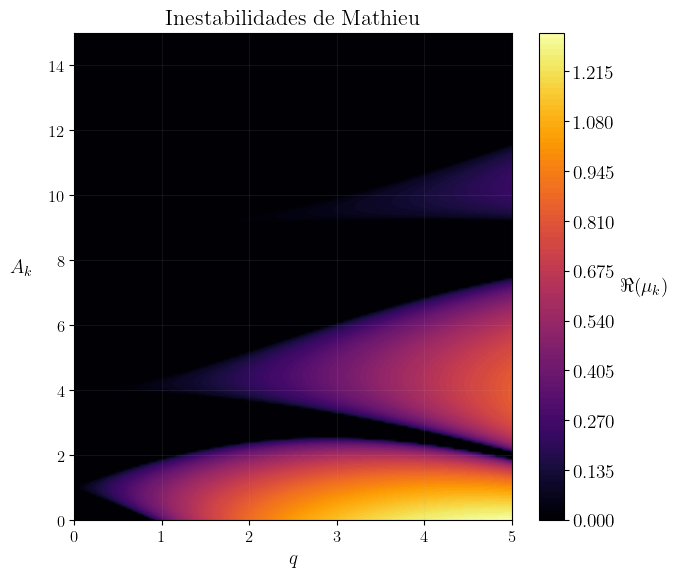
\includegraphics[width=1\linewidth]{Imagenes//Nahue/Mathieu_1.png}
        \caption{en esta imagen podemos ver cómo son las bandas para valores de $q$ entre 0 y 5, y valores de $A_k$ entre 0 y 15. Esta imagen es la misma que aparece en el texto de Mishra.}
        \label{fig:Mathieu1}
    \end{figure}
\end{minipage} \hfill
\begin{minipage}{0.45\textwidth}
    \begin{figure}[H]
        \centering
        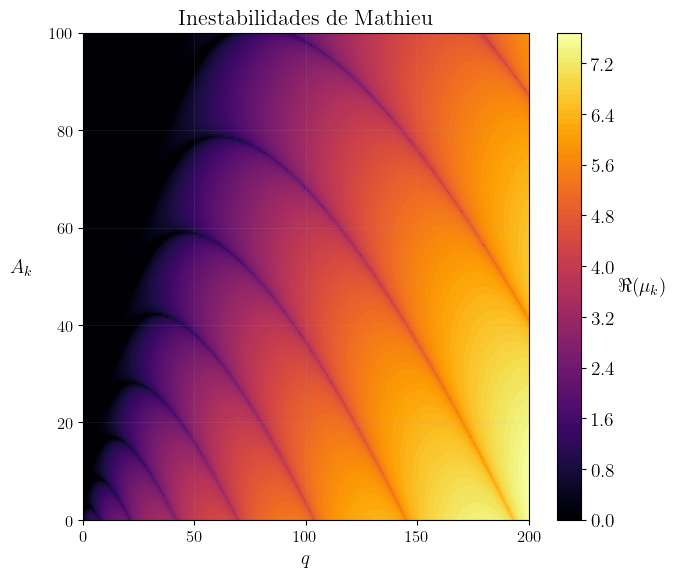
\includegraphics[width=1\linewidth]{Imagenes//Nahue/Mathieu_2.png}
        \caption{en esta imagen podemos ver cómo son las bandas para valores de $q$ entre 0 y 200, y valores de $A_k$ entre 0 y 100.}
        \label{fig:Mathieu2}
    \end{figure}
\end{minipage}

Ya que tenemos las bandas dónde hay inestabilidad, utilizando que $\displaystyle A_k = \left( \frac{k}{m} \right)^2  + 2 q$ podemos fijar $q$ y variar el modo para ver cómo se comporta la oscilación para distintos modos y ver qué tipo de resonancia tenemos, ésto lo podemos ver en las figuras \ref{fig:Mathieu3} y \ref{fig:Mathieu4}.

\begin{figure}[H]
    \centering
    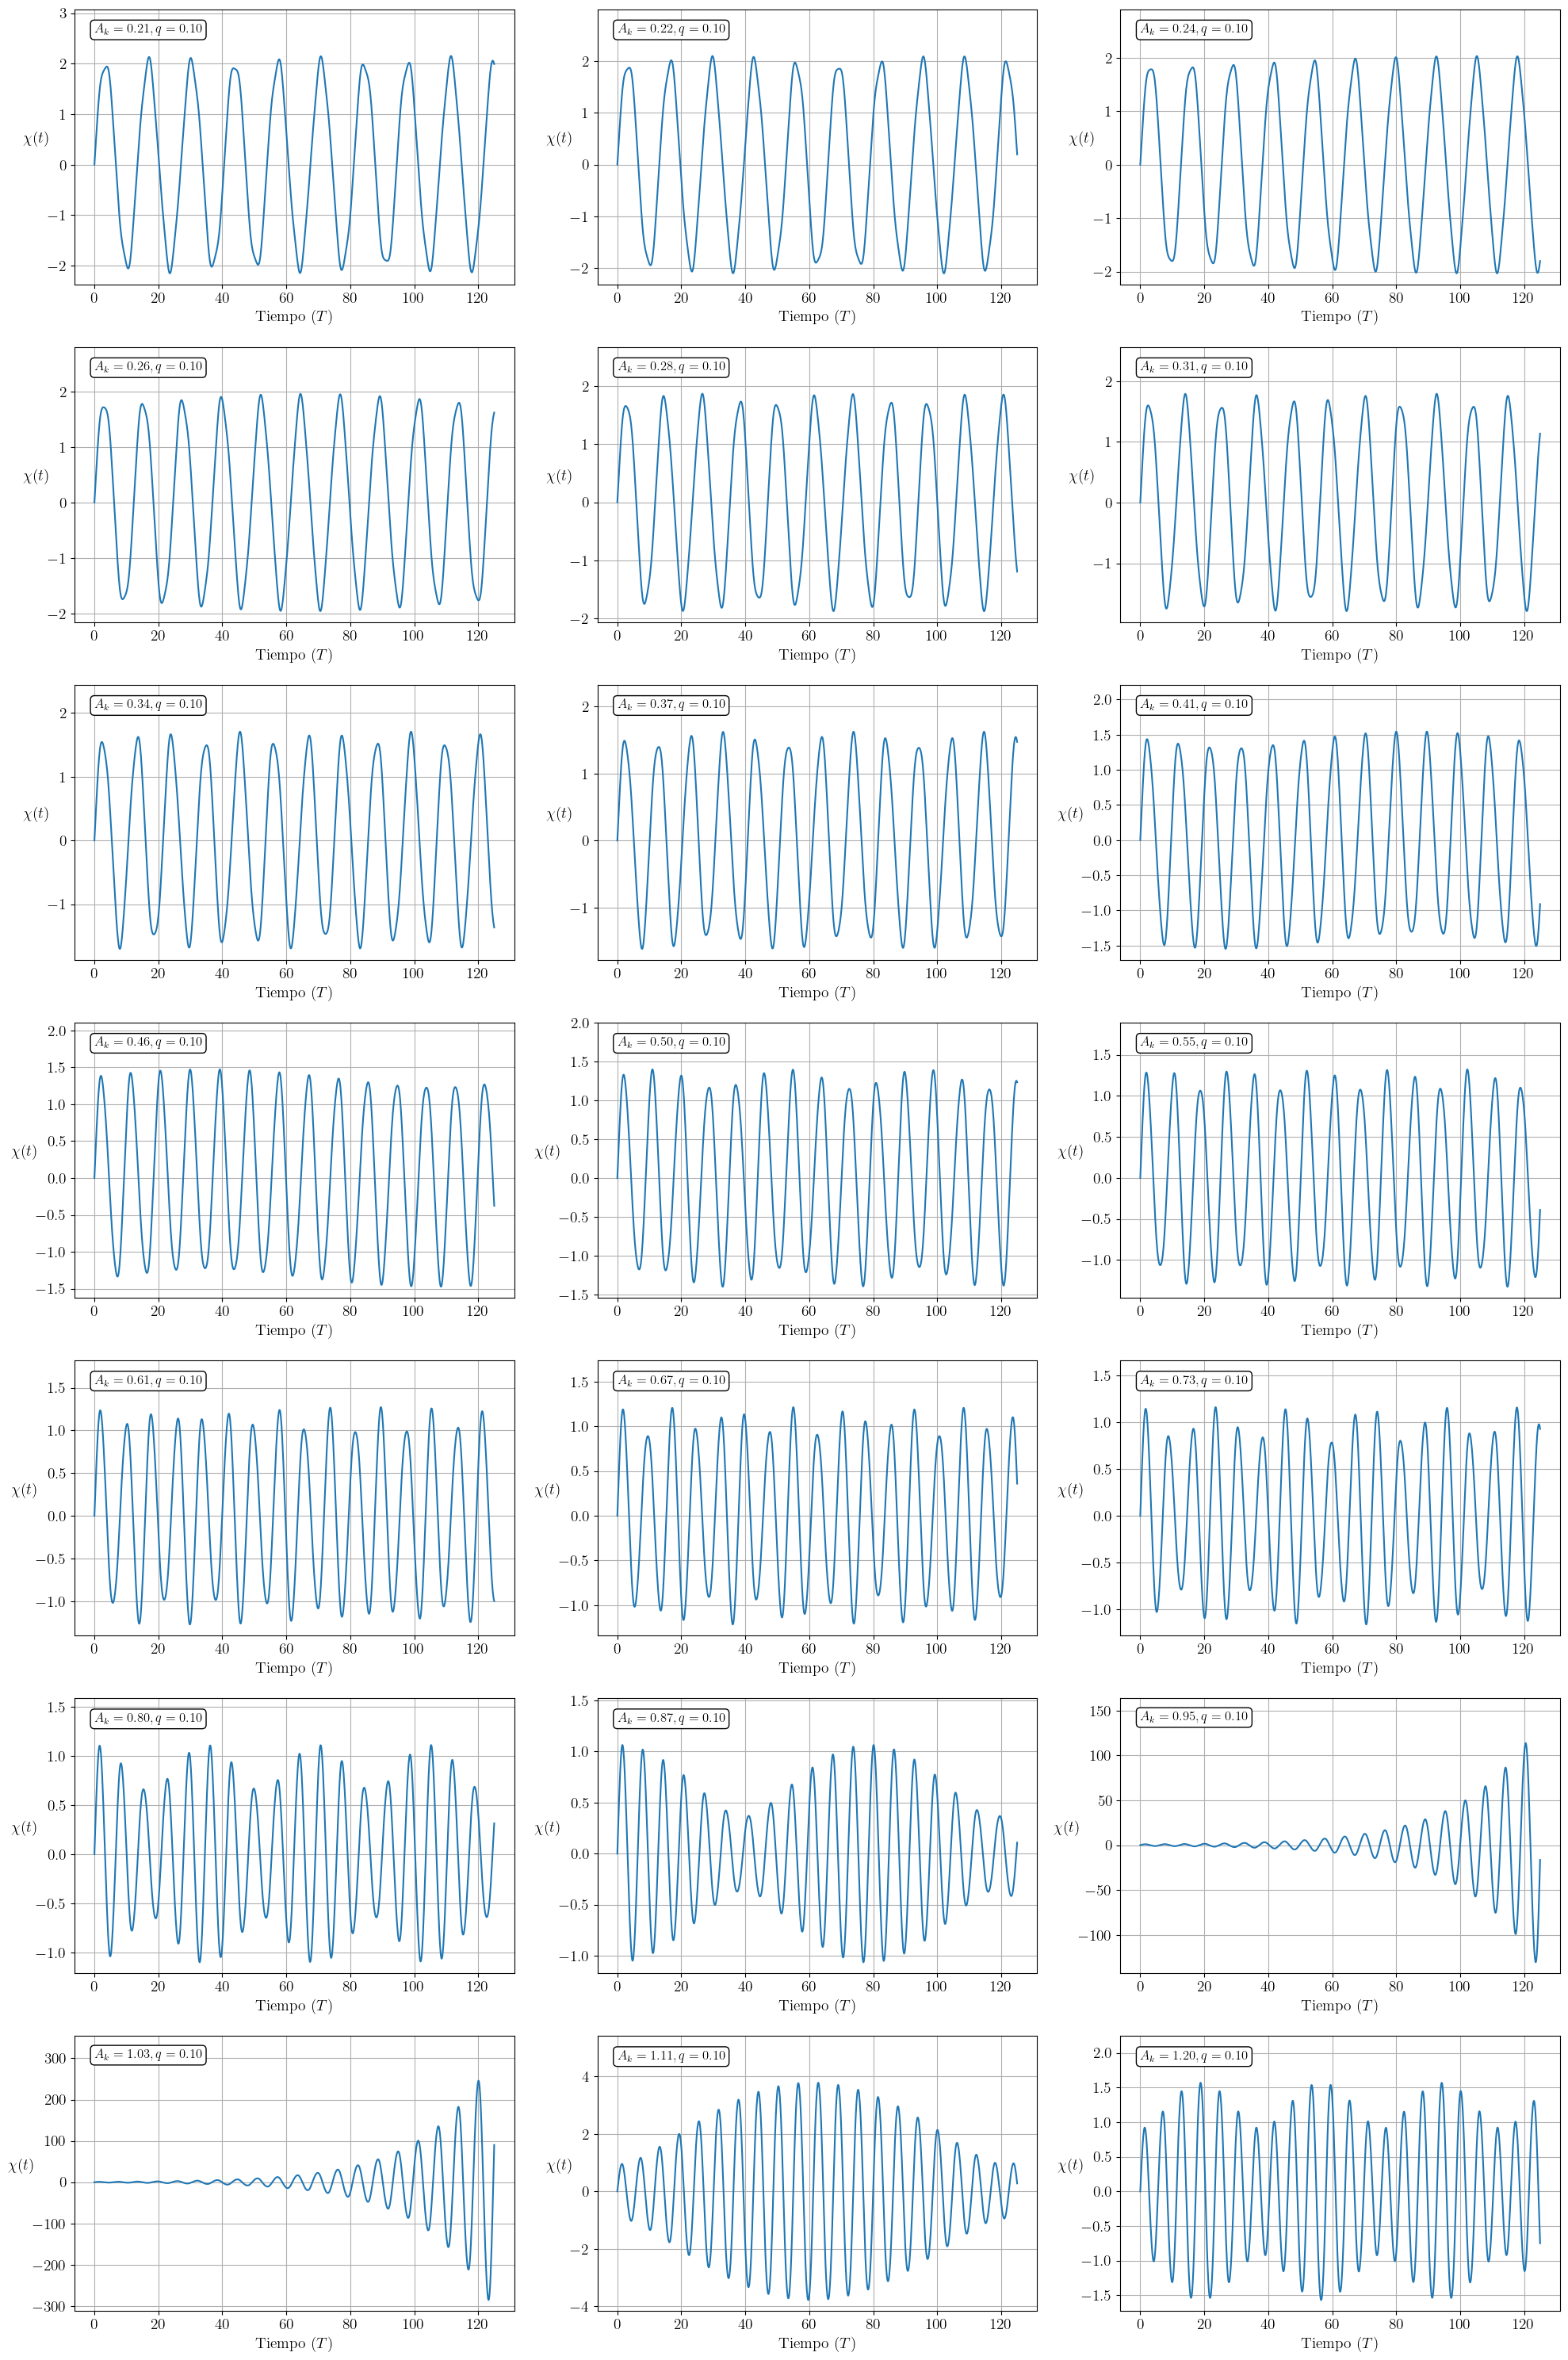
\includegraphics[width=0.9\linewidth]{Imagenes//Nahue/Mathieu_3.png}
    \caption{\centering en esta imagen vemos cómo evolucionan las soluciones de la ecuación de Mathieu para distintos modos con $q = 0.1$ (narrow resonance).}
    \label{fig:Mathieu3}
\end{figure}

\begin{figure}[H]
    \centering
    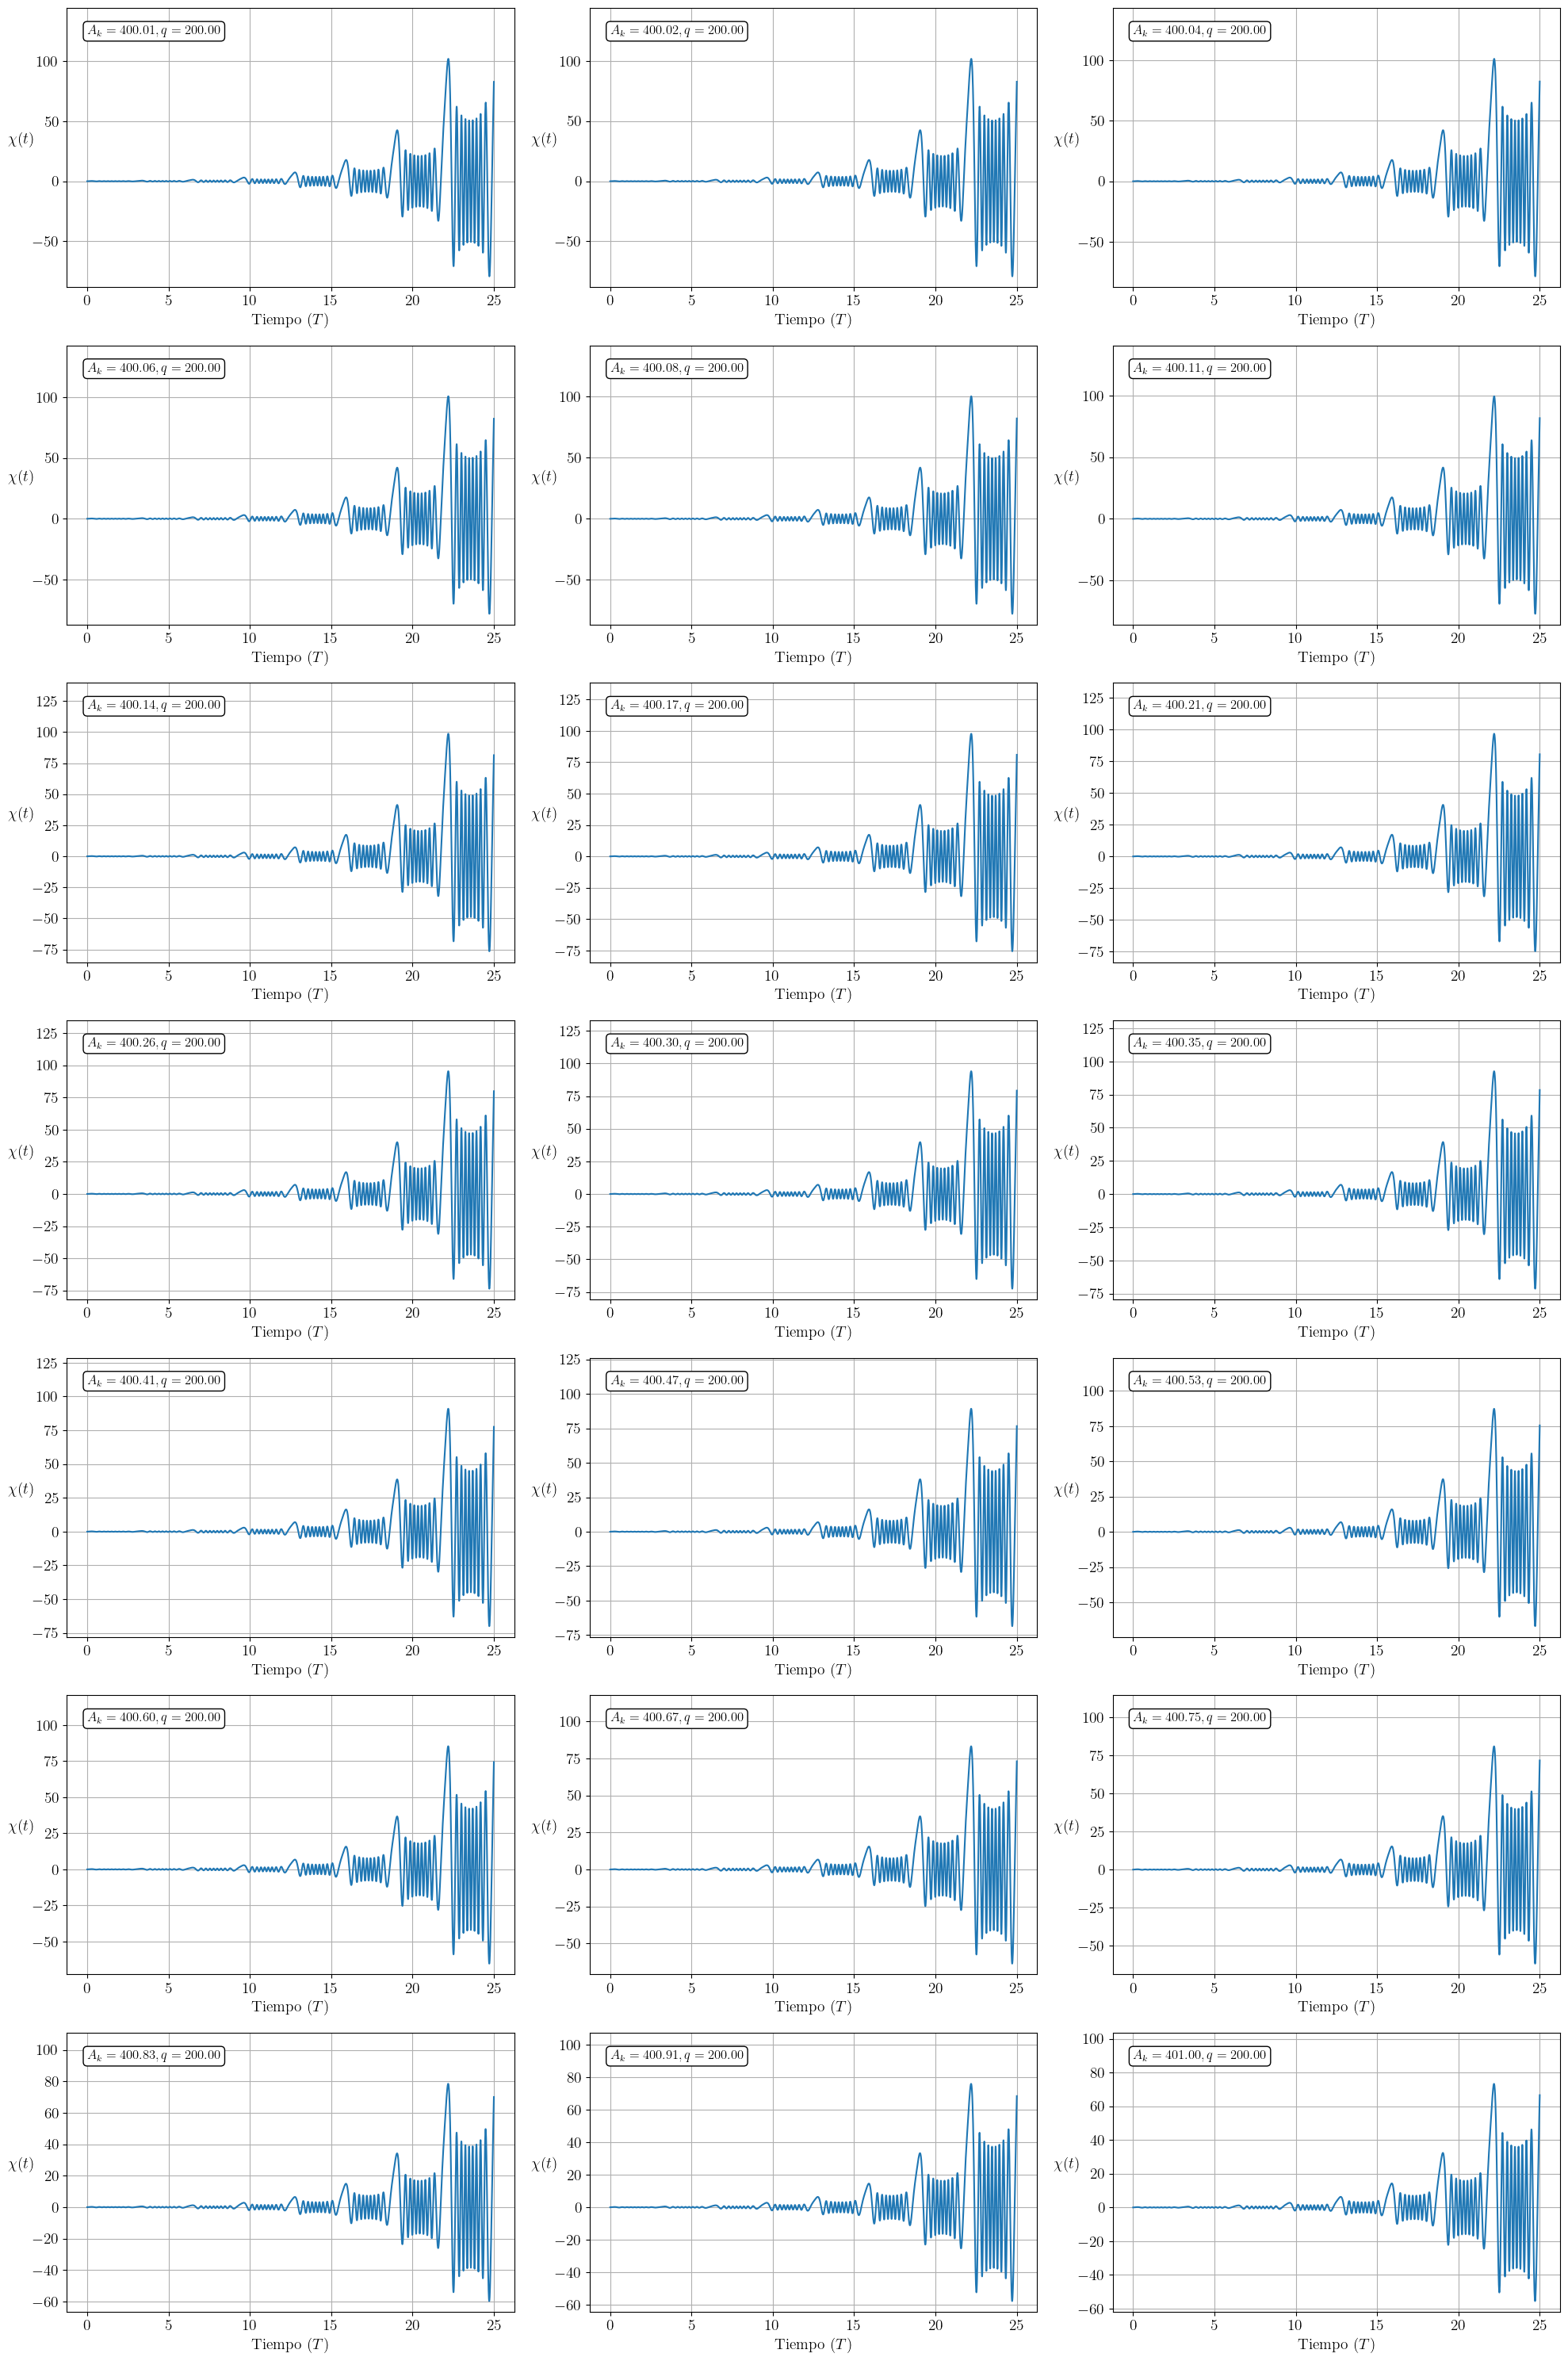
\includegraphics[width=0.9\linewidth]{Imagenes//Nahue/Mathieu_4.png}
    \caption{\centering en esta imagen vemos cómo evolucionan las soluciones de la ecuación de Mathieu para distintos modos con $q = 200$ (broad resonance).}
    \label{fig:Mathieu4}
\end{figure}

De las figuras \ref{fig:Mathieu3} y \ref{fig:Mathieu4} podemos buscar quedarnos con un gráfico de cada uno para ver cómo son los tipos de resonancias, en particular por la forma en que evolucionan los modos del campo hijo tomemos para $q = 0.1$ el valor de $A_k = 1.03$ y para $q = 200$ el valor de $A_k = 401$. Estos dos gráficos los podemos poner en \ref{fig:Mathieu5} y \ref{fig:Mathieu6} respectivamente.

\begin{minipage}{0.45\textwidth}
    \begin{figure}[H]
        \centering
        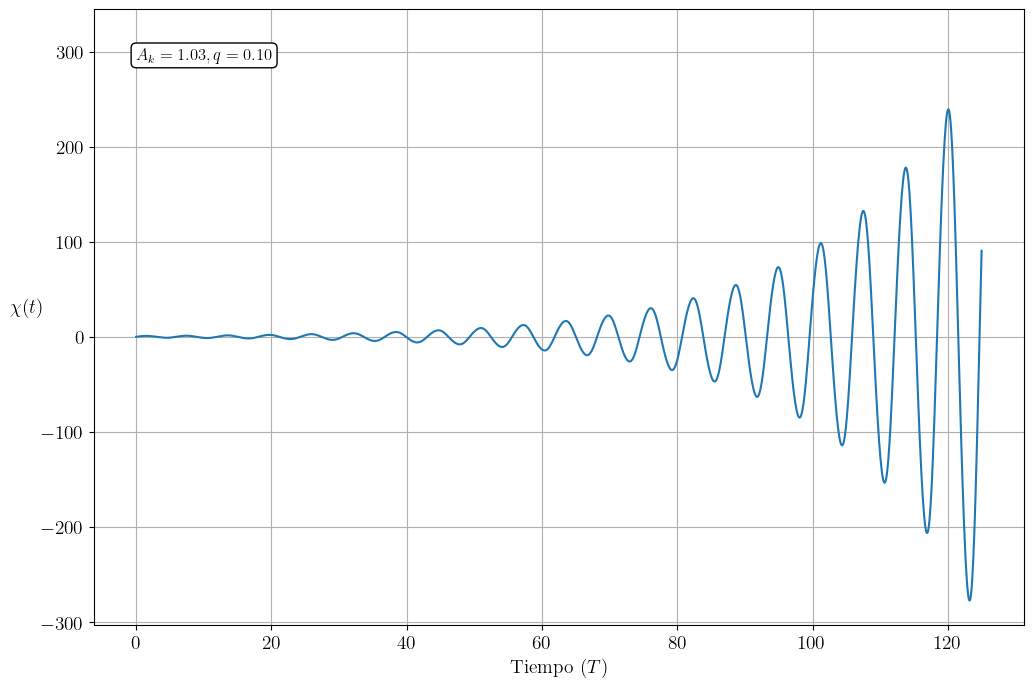
\includegraphics[width=1\linewidth]{Imagenes//Nahue/Mathieu_5.png}
        \caption{en esta imagen tenemos la evolución del modo con $q = 0.1$ y $A_k = 1.03$ lo que nos da una narrow resonance}
        \label{fig:Mathieu5}
    \end{figure}
\end{minipage} \hfill
\begin{minipage}{0.45\textwidth}
    \begin{figure}[H]
        \centering
        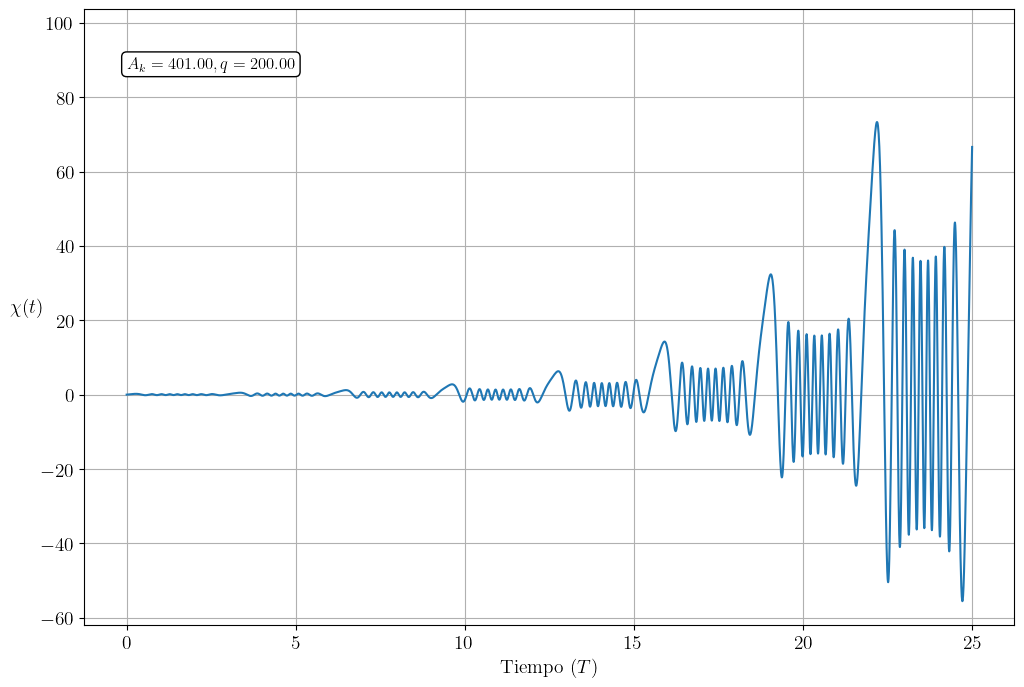
\includegraphics[width=1\linewidth]{Imagenes//Nahue/Mathieu_6.png}
        \caption{en esta imagen tenemos la evolución del modo con $q = 200$ y $A_k = 401$ lo que nos da una narrow resonance}
        \label{fig:Mathieu6}
    \end{figure}
\end{minipage}

Con estos valores de $q$ y $A_k$ podemos calcular el número de partículas producidas, lo cual lo haremos usando 

\begin{equation}
    n_\chi (k) = \frac{1}{2 \Omega_\chi} \left( \left| \frac{d \chi_k}{dT} \right|^2 + \Omega^2_\chi \left| \chi_k \right|^2 \right) - \frac{1}{2}
\end{equation}

\noindent
siendo

\begin{equation}
    \Omega_\chi^2 (k, t) = \frac{k^2}{a^2} + g^2 \phi^2 (t)
\end{equation}

\noindent
y el campo $\phi (t) = \phi_0 \sin (T)$. Entonces debemos definir parámetros para $g$, $a$ y $\phi_0$ y con ésto obtenemos las figuras \ref{fig:Mathieu7} para narrow resonance y \ref{fig:Mathieu8} para broad resonance. Para estos gráficos tomamos $a = 1$, $g = 10^{-14}$ y $\phi_0 = 1$.

\begin{minipage}{0.45\textwidth}
\begin{figure}[H]
    \centering
    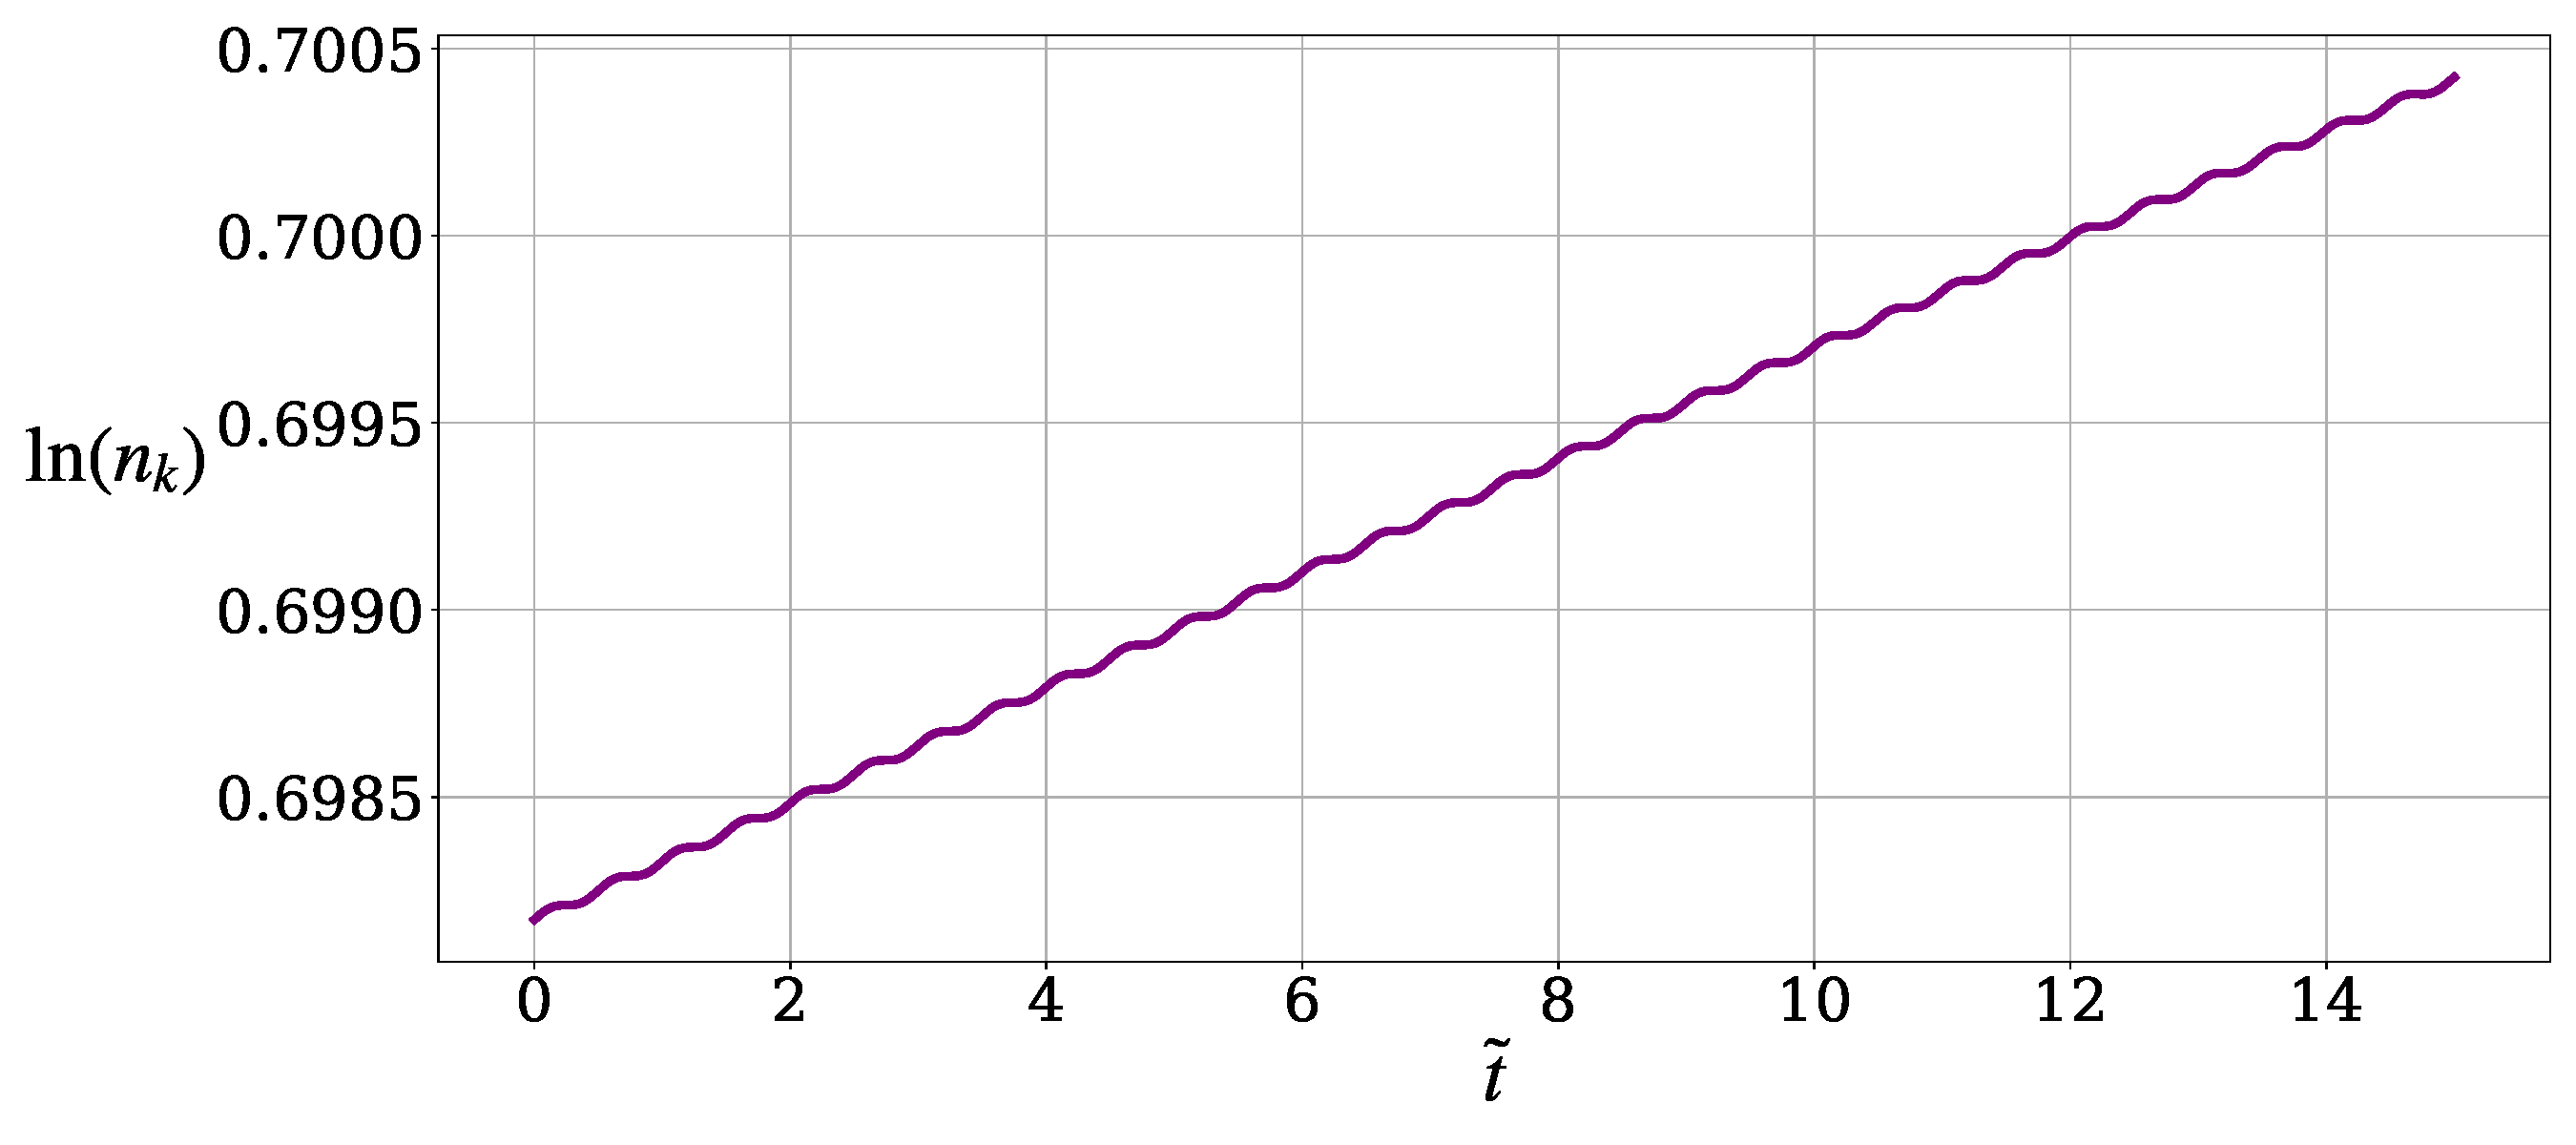
\includegraphics[width=1\linewidth]{Imagenes//Nahue/Narrow_resonance.pdf}
    \caption{número de partículas para narrow resonance. Para esta figura tomamos $q = 0.1$ y $A_k = 1.03$.}
    \label{fig:Mathieu7}
\end{figure}
\end{minipage} \hfill
\begin{minipage}{0.45\textwidth}
    \begin{figure}[H]
        \centering
        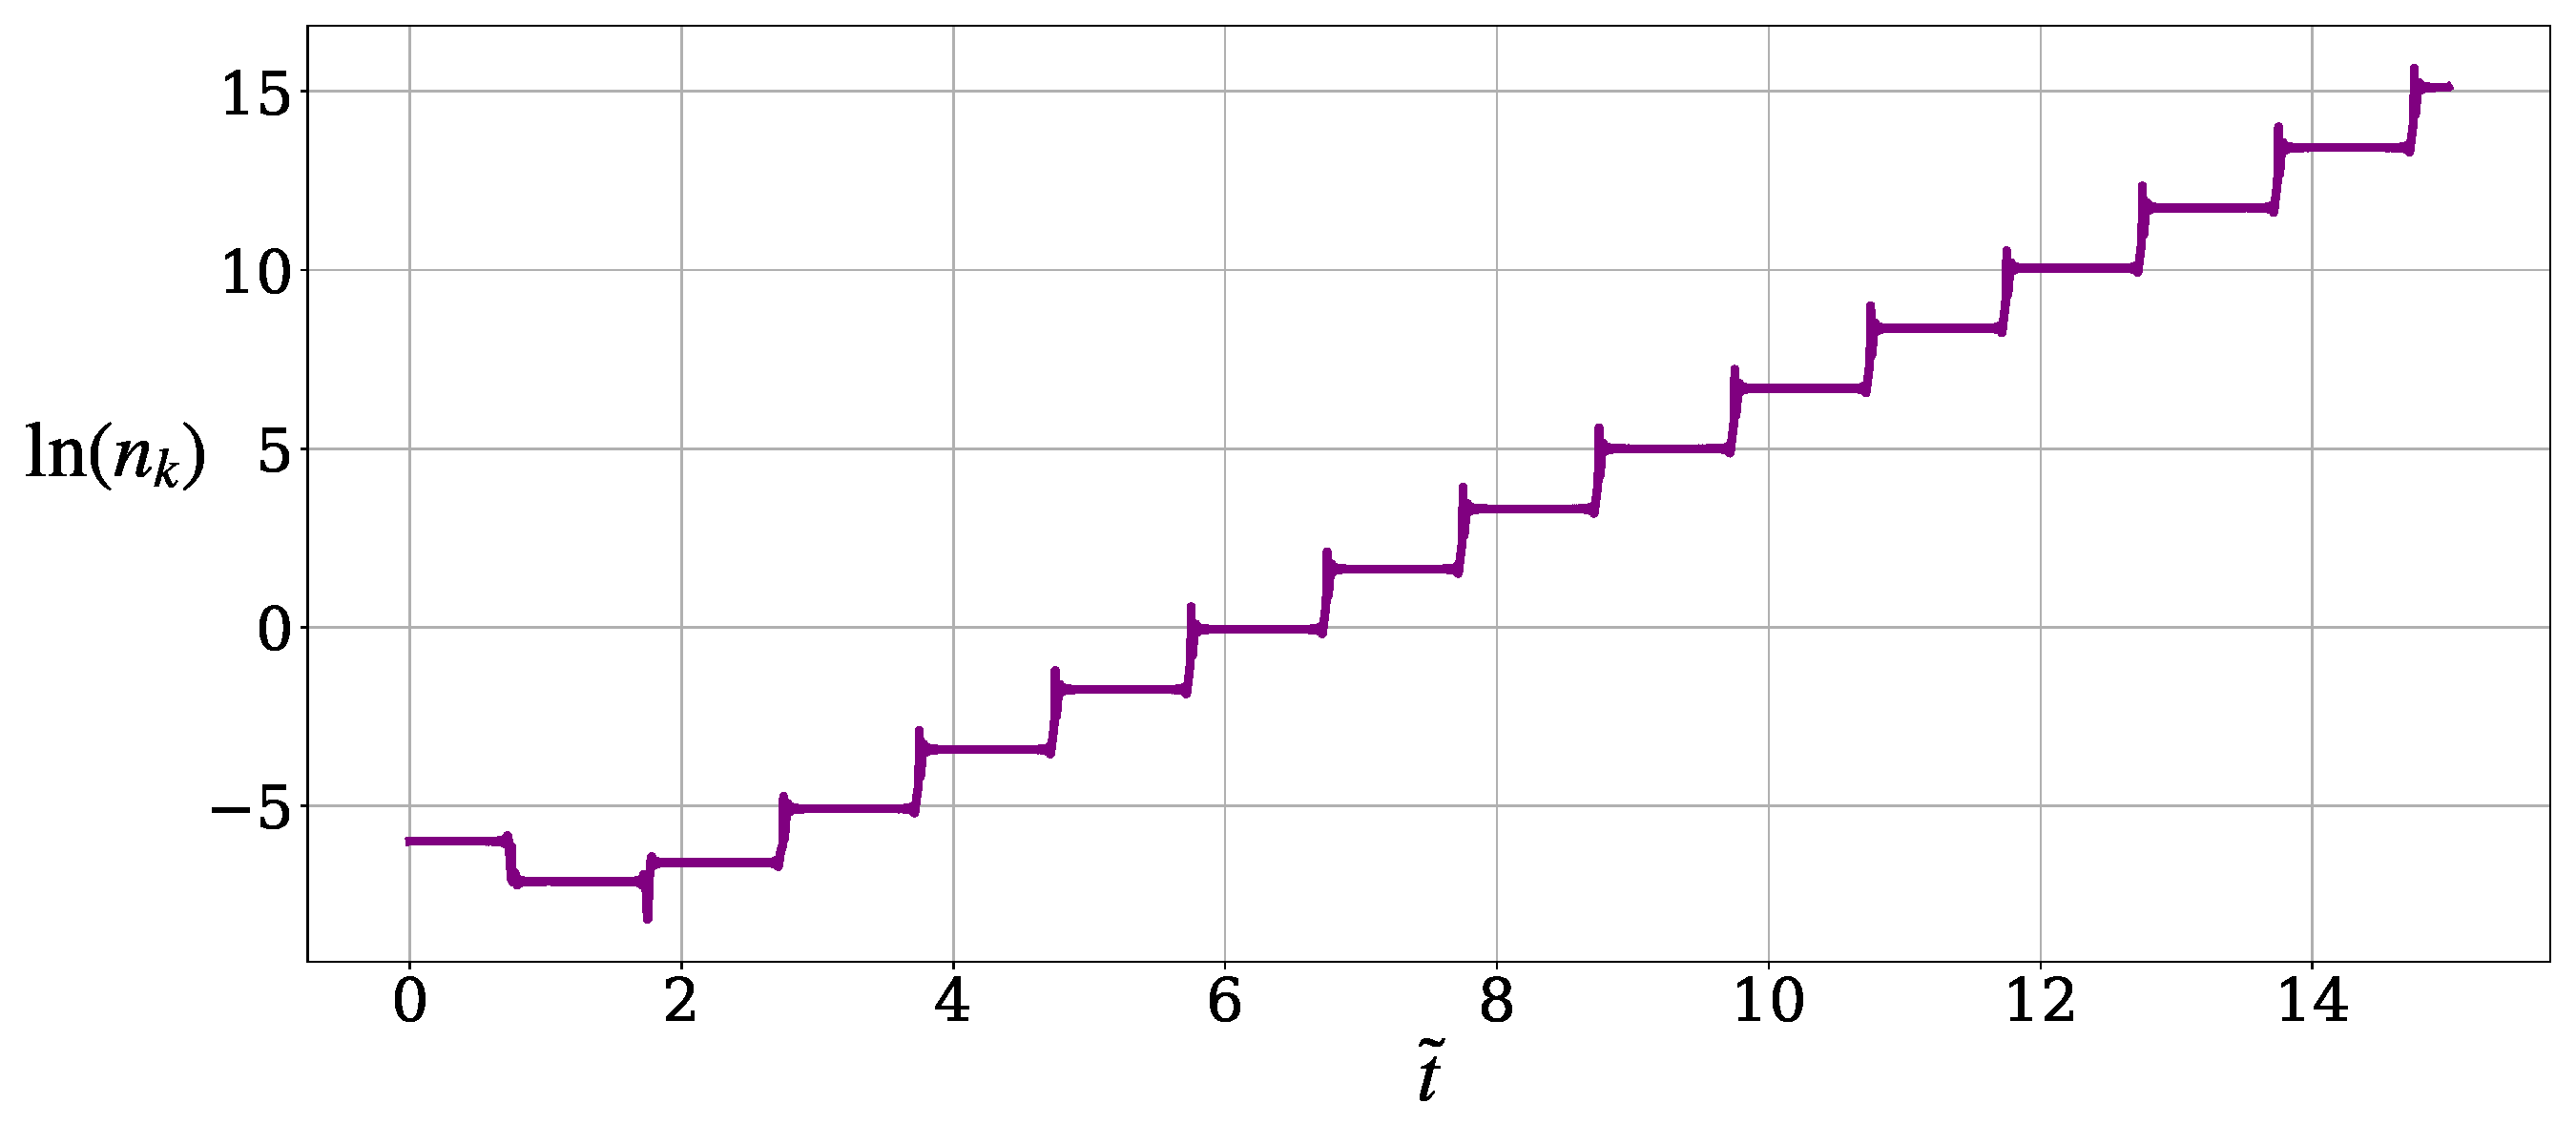
\includegraphics[width=1\linewidth]{Imagenes//Nahue/Broad_resonance.pdf}
        \caption{número de partículas para broad resonance. Para esta figura tomamos $q = 200$ y $A_k = 401$.}
        \label{fig:Mathieu8}
    \end{figure}
\end{minipage}

\subsection{Floquet}

Un análisis de Floquet nos permite ver las bandas dónde la resonancia paramétrica dá inestabilidades, este análisis lo podemos hacer a partir de la matriz de monodromía que se encuentra descripta en el paper arXiv:1410.3808. A partir de esto mismo se armaron los códigos que se encuentran en \href{https://github.com/TomasCiccarella/Tesis/blob/master/Floquet/Floquet.ipynb}{Floquet.ipynb} y se armaron las figuras \ref{fig:Floquet_m2phi2} y \ref{fig:Floquet_lphi4}. Estas figuras se pueden comparar con la tabla de inestabilidades de Mathieu que armamos previamente y con la tabla de inestabilidades que se puede observar en \textit{Parametric Resonance in the Early Universe - A Fitting Analysis} viendo que efectivamente el código que armamos es correcto.

Para armar la matriz de monodromía es necesario definir un período de oscilación que lo podemos obtener a partir de la conservación de la energía y lo realizado en \ref{Periodo_Floquet}.

\begin{figure}[H]
    \begin{subfigure}[t]{0.5\linewidth}
        \centering
        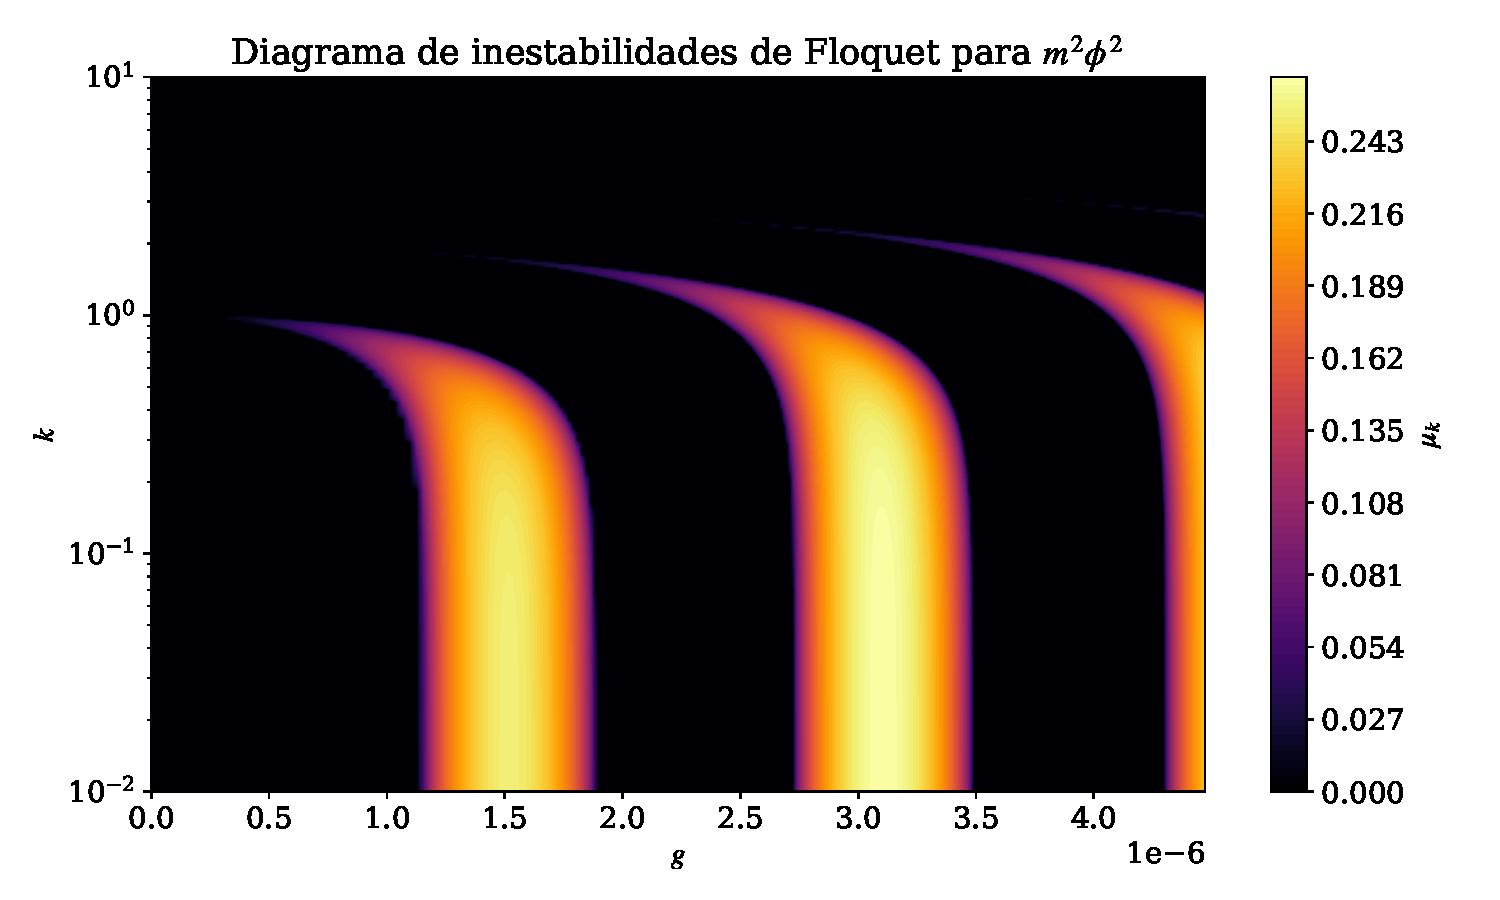
\includegraphics[width = \linewidth]{Imagenes/Nahue/Floquet_m2phi2.pdf}
        \caption{$m^2 \phi^2$}
        \label{fig:Floquet_m2phi2}
    \end{subfigure}
    \begin{subfigure}[t]{0.5\linewidth}
        \centering
        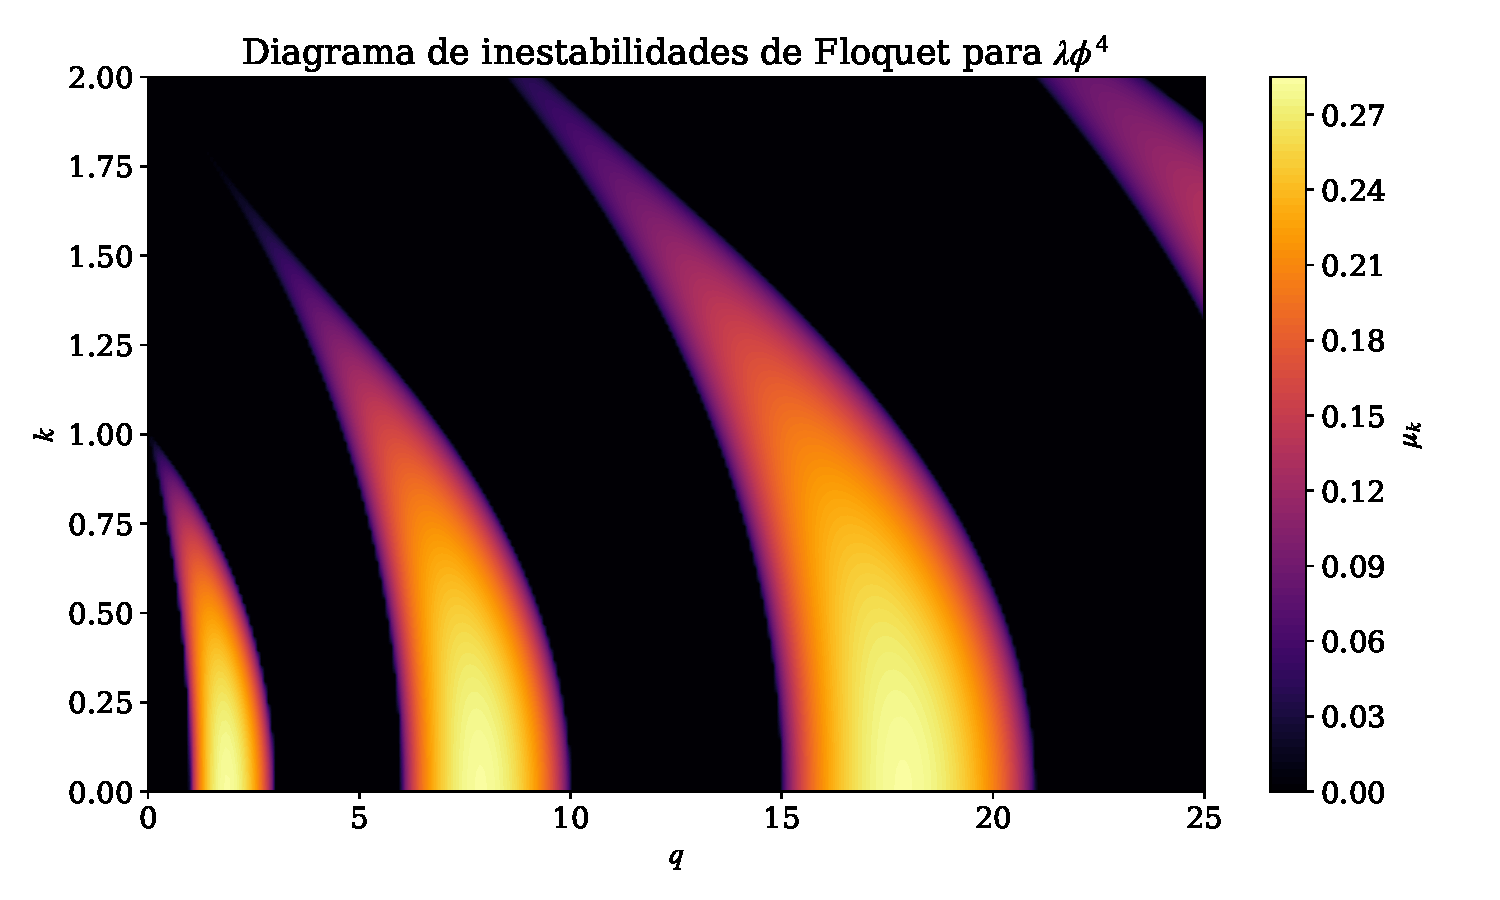
\includegraphics[width = \linewidth]{Imagenes/Nahue/Floquet_lphi4.pdf}
        \caption{$\lambda \phi^4$}
        \label{fig:Floquet_lphi4}
    \end{subfigure}
    \caption{tabla de inestabilidades de Floquet, armados a partir de la ecuación de Mathieu y Lamé.}
\end{figure}

Una vez que tenemos las tablas de inestabilidades, podemos dejar fijo un valor de $q$ y vér cómo se comporta en $k$ ya que más adelante nos gustaría poder comparar si la banda de amplificación que obtenemos con el análisis por Floquet es la banda de amplificación para el espectro de potencias y para el espectro de ondas gravitacionales, entonces con esta idea en mente armamos las figuras \ref{fig:mu_m2phi2} y \ref{fig:mu_lphi4} que representan cómo varía el parámetro de Floquet $\mu_k$ con respecto al número de onda $k$ para un $q$ fijo.

\begin{figure}[H]
    \begin{subfigure}[t]{0.5\linewidth}
        \centering
        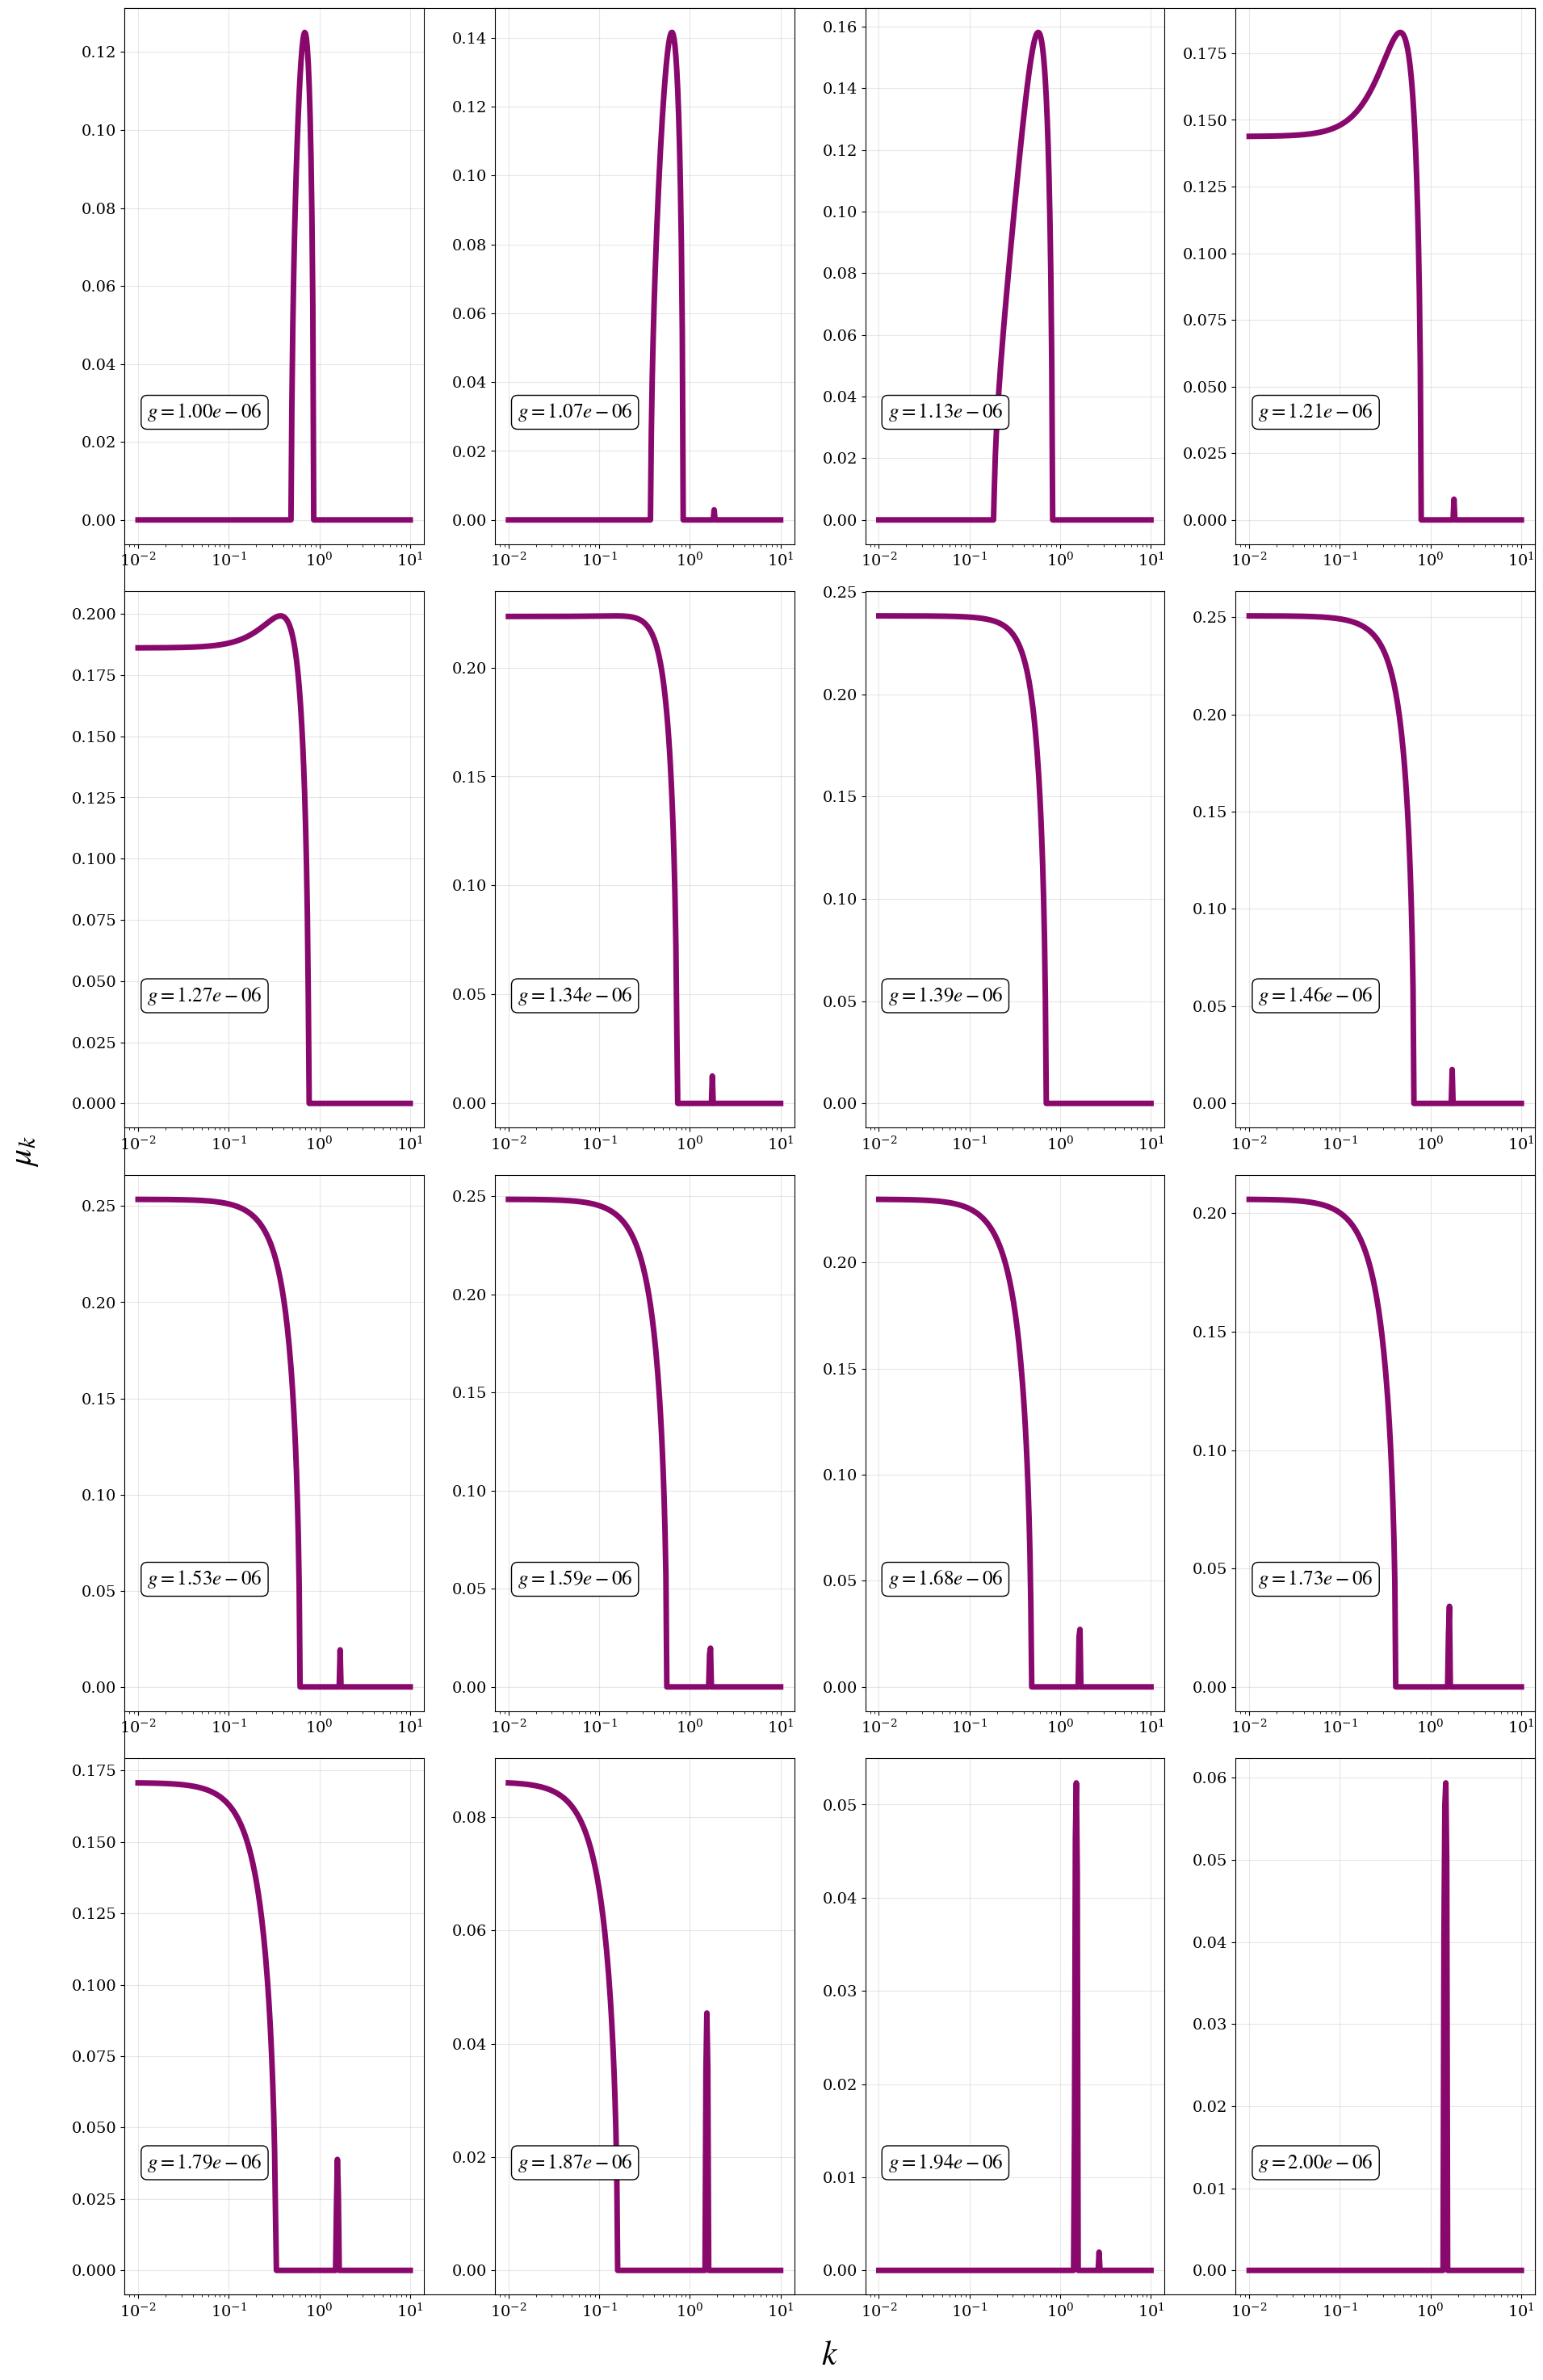
\includegraphics[width = \linewidth]{Imagenes/Nahue/mu_m2phi2.png}
        \caption{$m^2 \phi^2$}
        \label{fig:mu_m2phi2}
    \end{subfigure}
    \begin{subfigure}[t]{0.5\linewidth}
        \centering
        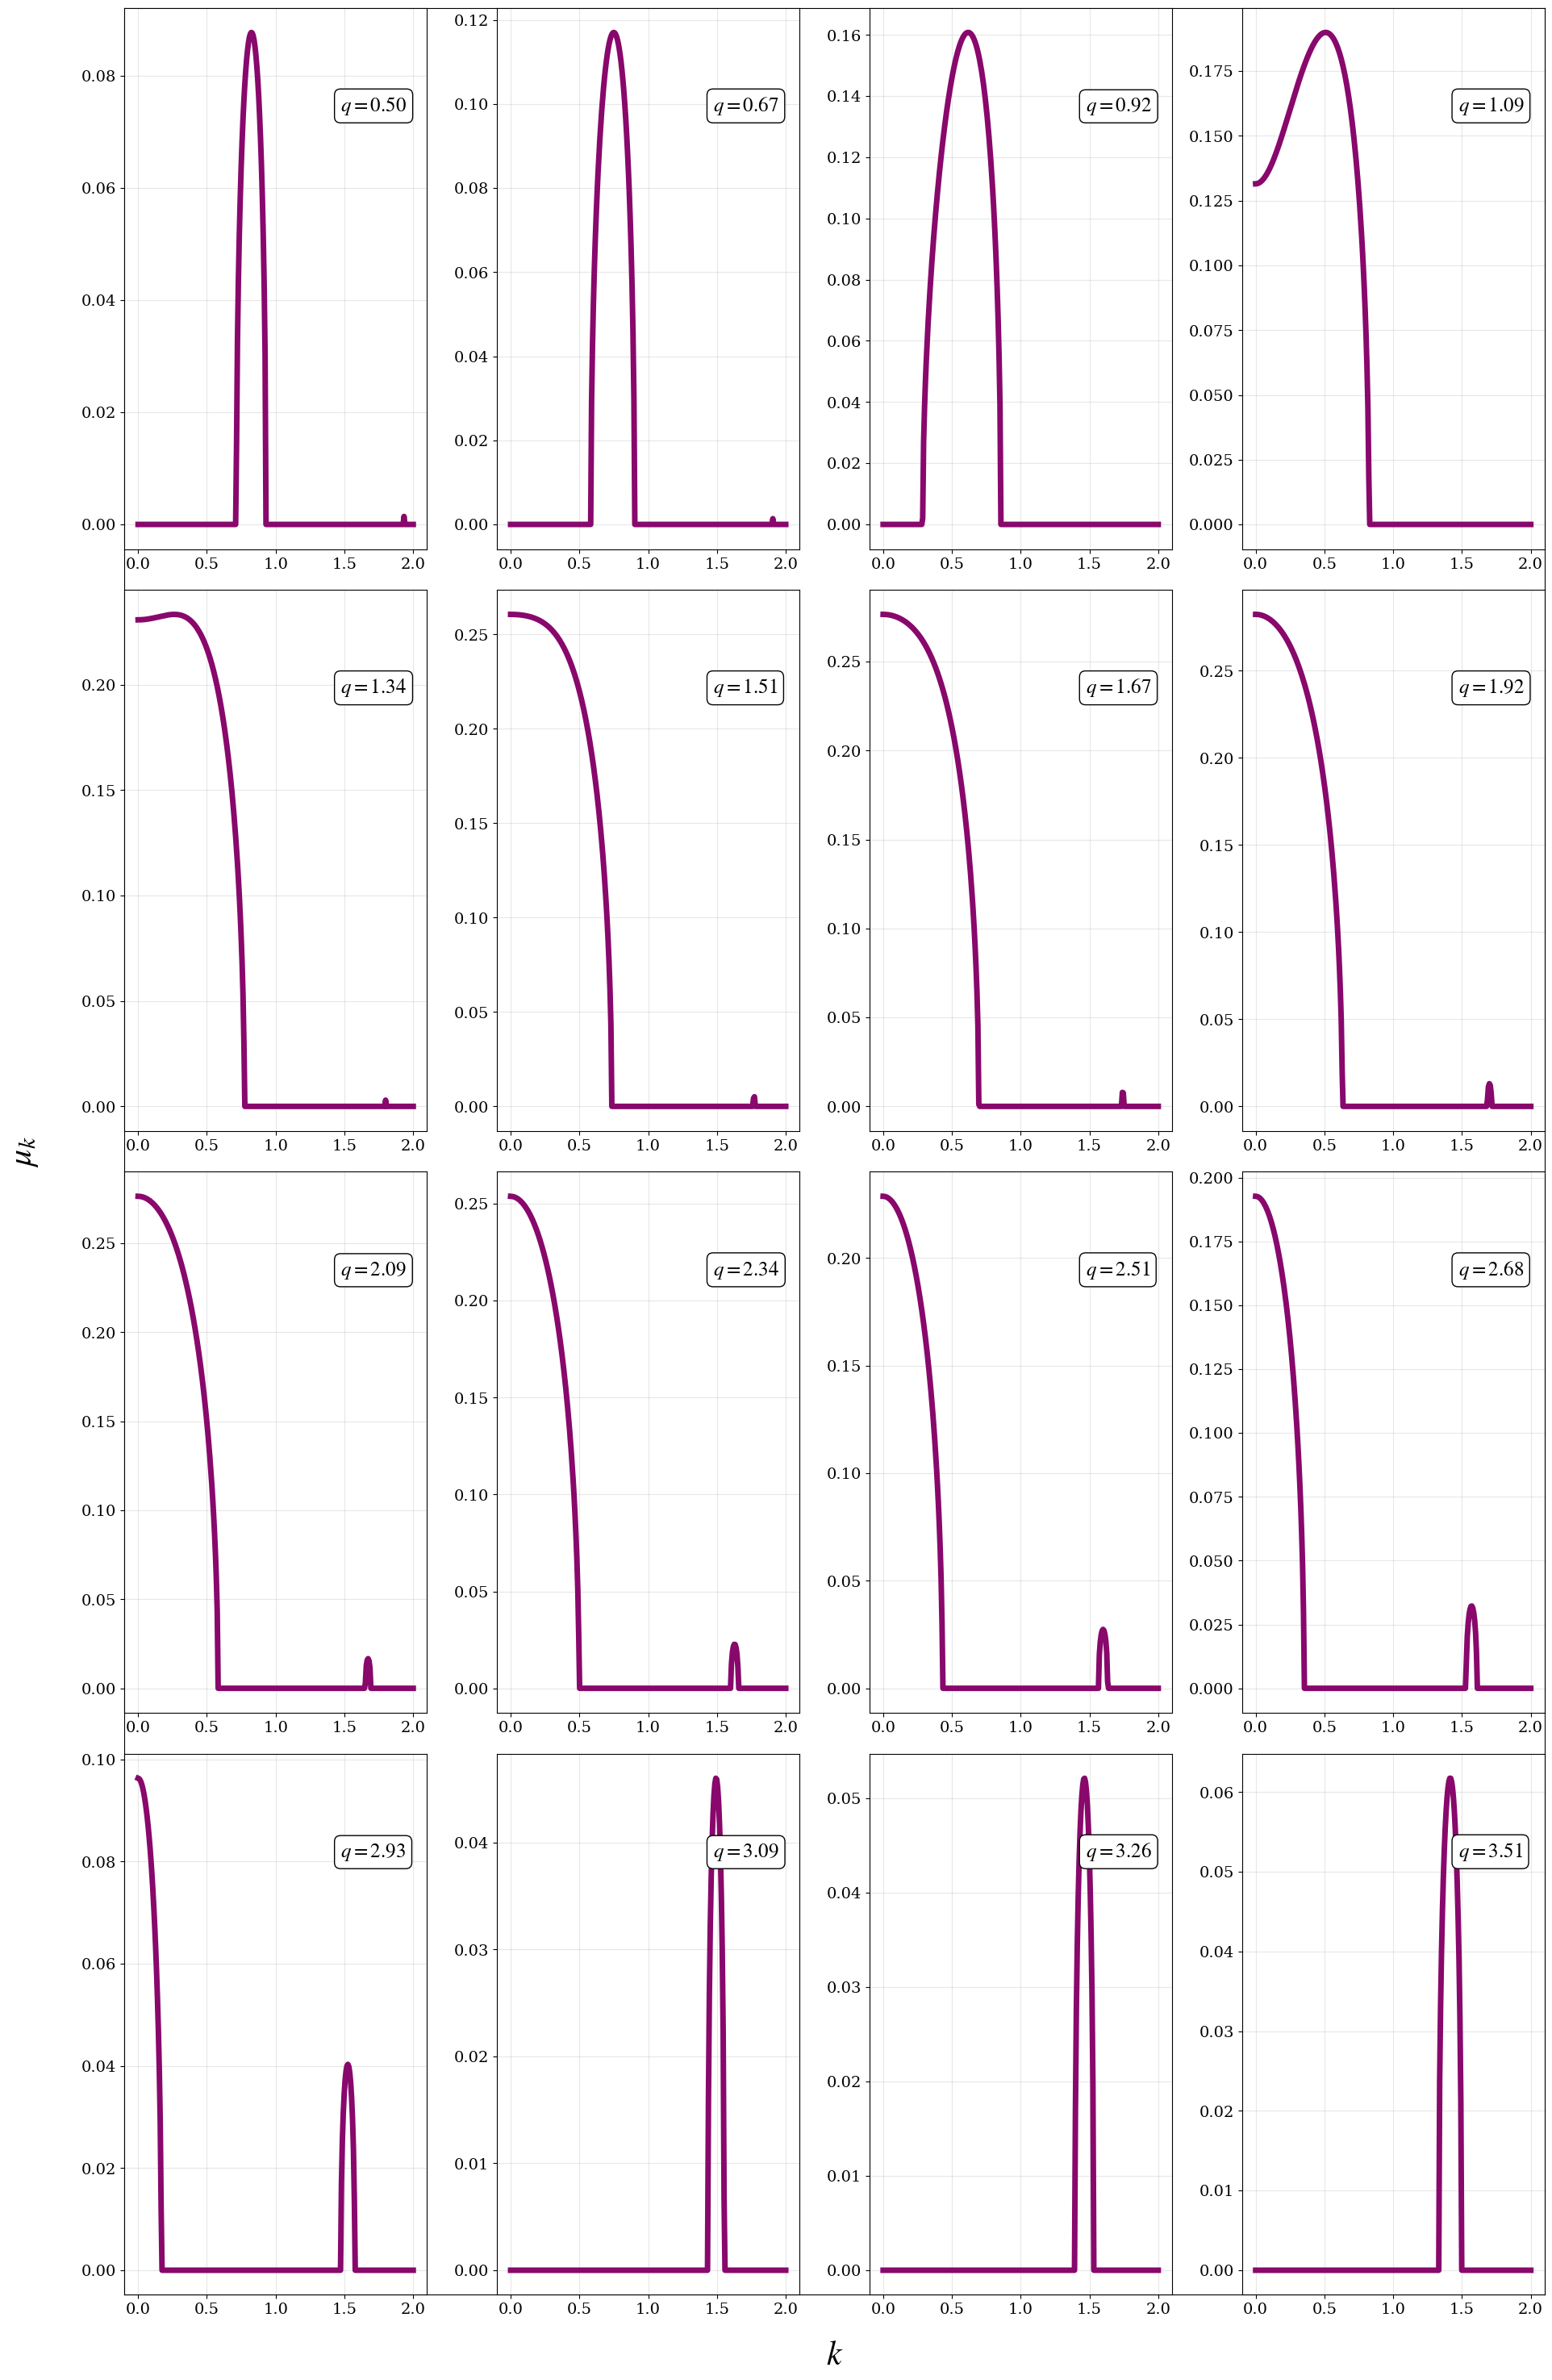
\includegraphics[width = \linewidth]{Imagenes/Nahue/mu_lphi4.png}
        \caption{$\lambda \phi^4$}
        \label{fig:mu_lphi4}
    \end{subfigure}
    \caption{variación del parámetro de Floquet con el número de onda.}
\end{figure}

\subsection{Modelo de $\lambda \phi^4$}

Para un modelo $\lambda \phi^4$, las ecuaciones lineales que describen la dinámica de los campos son:

\begin{equation}
    \begin{cases}
        \displaystyle \frac{d^2 \tilde{\phi}}{d \tilde{t}^2} + \frac{3}{a} \frac{d a}{d \tilde{t}} \frac{d \tilde{\phi}}{d \tilde{t}} + \tilde{\phi}^3 &= 0  \\ \\
        \displaystyle \frac{d^2 a}{d \tilde{t}^2} + \frac{a}{3} \left[ \left( \frac{d \tilde{\phi}}{d \tilde{t}} \right)^2 - \frac{\tilde{\phi}^4}{4} \right] &= 0
    \end{cases}
\end{equation}

\begin{equation}
  \begin{cases}
    \displaystyle \frac{d^2 \delta \tilde{\phi}_k}{d \tilde{t}^2} + \frac{3}{a} \frac{d a}{d \tilde{t}} \frac{d \tilde{\phi}_k}{d \tilde{t}} + \left( \frac{\tilde{k}^2}{a^2} + 3 \tilde{\phi}^2 \right) \delta \tilde{\phi}_k &= 0\\ \\
    \displaystyle \frac{d^2 \tilde{\chi}_k}{d \tilde{t}^2} + \frac{3}{a} \frac{d a}{d \tilde{t}} \frac{d \tilde{\chi}_k}{d \tilde{t}} + \left( \frac{\tilde{k}^2}{a^2} + g^2 \tilde{\phi}^2 \right) \tilde{\chi}_k &= 0
    \end{cases}
\end{equation}

\noindent
siendo las primeras las ecuaciones para el background y las últimas para las perturbaciones

Ahora las condiciones iniciales para $V(\phi) = \lambda \phi^4$ las podemos calcular a partir de la misma idea y nos van a quedar que para los campos tenemos:

\begin{equation*}
    \begin{split}
        \frac{m_p^2}{16 \pi} \left( \frac{\lambda \phi_0^3}{\displaystyle \frac{1}{4} \lambda \phi_0^4} \right)^2 &\approx 1\\
        \frac{m_p^2}{16 \pi} \cdot \frac{16}{\phi_0^2} &\approx 1\\
        \phi_0^2 \approx \frac{m_p^2}{\pi}
    \end{split}
\end{equation*}

\begin{equation}
    \phi_0 \approx \frac{m_p}{\sqrt{\pi}}
\end{equation}

\begin{equation*}
    \begin{split}
        \frac{1}{2} \dot{\phi}^2_0 &\approx V(\phi_0)\\
        \dot{\phi}^2_0 &\approx \frac{1}{2} \lambda \phi_0^4
    \end{split}
\end{equation*}

\begin{equation}
    \dot{\phi}_0 \approx \sqrt{\frac{\lambda}{2}} \phi_0^2
\end{equation}

\noindent
para el caso de las condiciones iniciales para la expansión del universo como $a$ está definida de forma comparativa por tanto podemos considerar $a_{reh} = 1$ y $\dot{a}_{reh}$ saldrá de ver la primera ecuación de Friedmann entonces tenemos

\begin{equation*}
    \begin{split}
        \frac{\dot{a}_{reh}^2}{a_{reh}^2} &= \frac{1}{3 m_p^2} \left[ \frac{1}{2} \dot{\phi}^2_0 + V(\phi_0) \right]\\
        \dot{a}_{reh}^2 &= \frac{a_{reh}^2}{3 m_p^2} \cdot \frac{1}{2} \lambda \phi^4_0
    \end{split}
\end{equation*}

\begin{equation}
    \dot{a}_{reh} \approx \frac{\lambda a_{reh}}{\sqrt{6} m_p} \phi_0^2    
\end{equation}

\subsubsection{Sin expansión}

A partir de estas condiciones iniciales y el diagrama de Floquet que armamos en la subsección pasada podemos analizar cómo es la dinámica para distintos parámetros $(k,q)$ obteniendo la resonancias narrow y broad que podemos ver en las figuras \ref{fig:lphi4_narrow} y \ref{fig:lphi4_broad} que se obtenieron a partir de armar gráficos del estilo \ref{fig:mu_lphi4} y buscar el valor máximo para $k$. Nuevamente, estas figuras las podemos comparar con \textit{Parametric Resonance in the Early Universe - A Fitting Analysis} para poder ver que el código funciona correctamente.

\begin{figure}[H]
    \begin{subfigure}[t]{0.5\linewidth}
        \centering
        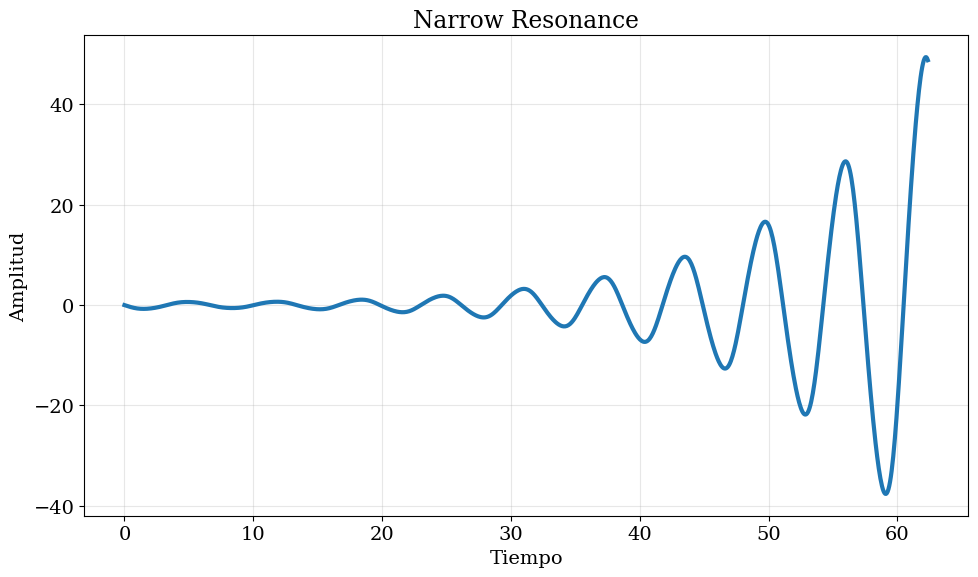
\includegraphics[width = \linewidth]{Imagenes/Nahue/lphi4_narrow.png}
        \caption{narrow resonance: $q = 0.5$ y $k = 0.8277856966198477$}
        \label{fig:lphi4_narrow}
    \end{subfigure}
    \begin{subfigure}[t]{0.5\linewidth}
        \centering
        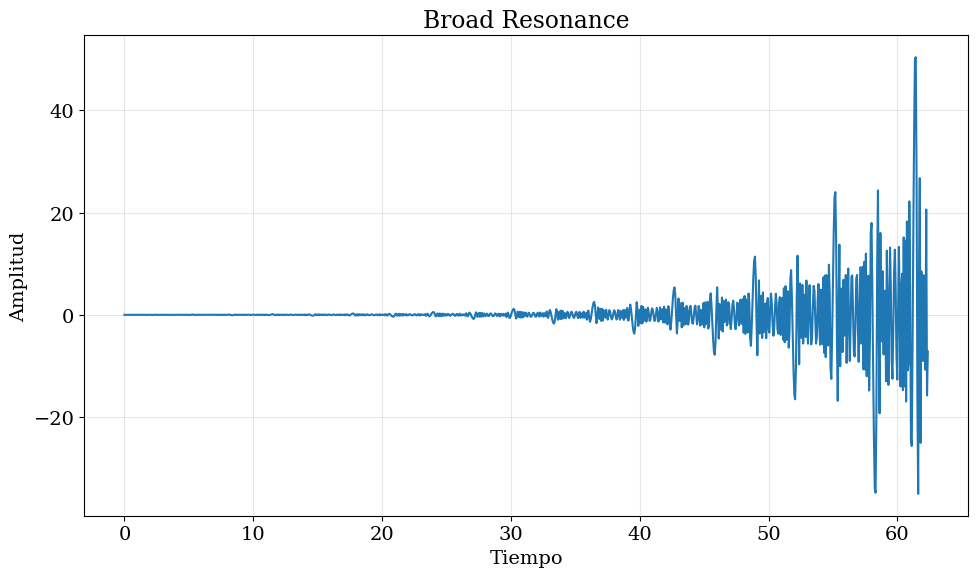
\includegraphics[width = \linewidth]{Imagenes/Nahue/lphi4_broad.png}
        \caption{broad resonance: $q = 5050$ y $k = 6.4686076615463275$}
        \label{fig:lphi4_broad}
    \end{subfigure}
    \caption{evolución de las resonancias en el tiempo.}
\end{figure}

Ya con la evolución de las perturbaciones podemos graficar el número de ocupación del campo que lo podemos calcular a partir de 

\begin{equation}
    n_\chi (k) = \frac{1}{2 \Omega_\chi} \left( \left| \frac{d \chi_k}{dT} \right|^2 + \Omega^2_\chi \left| \chi_k \right|^2 \right)
\end{equation}

\noindent
dónde $\displaystyle \Omega_\chi^2 (k, t) = \frac{k^2}{a^2} + g^2 \phi^2 (t)$ y depende del tipo de resonancia que tenemos se espera que el número de particulas oscile teniendo un comportamiento mayormente creciente (narrow resonance) o un número de partículas que oscile alrededor de una constante y que cada ciertos momentos tiene un \textit{burst} de partículas generando un salto abrupto en este valor. Ésto mismo lo podemos ver en las figuras \ref{fig:n_narrow} y \ref{fig:n_broad}, viendo que ocurre lo esperado.

\begin{figure}[H]
    \begin{subfigure}[t]{0.5\linewidth}
        \centering
        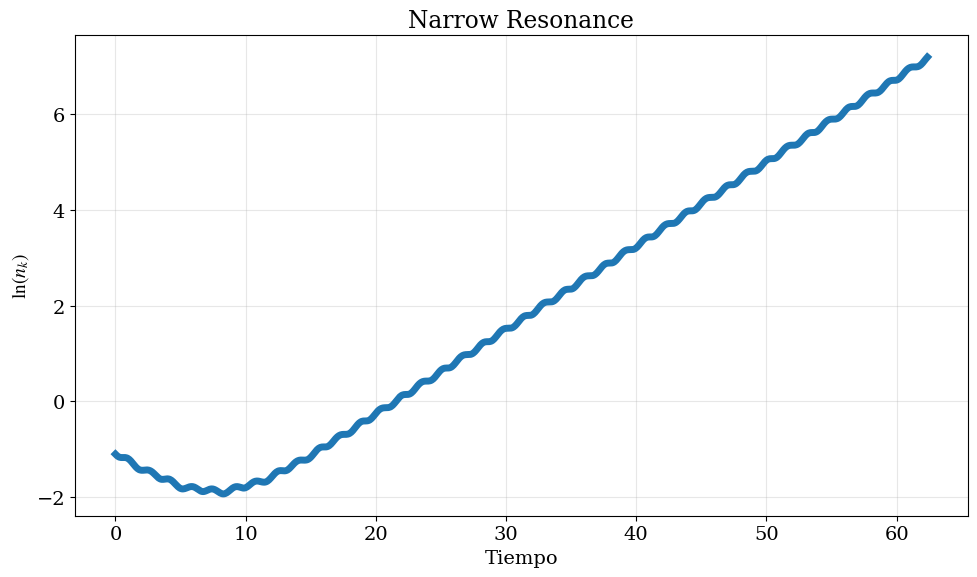
\includegraphics[width = \linewidth]{Imagenes/Nahue/n_narrow.png}
        \caption{narrow resonance: $q = 0.5$ y $k = 0.8277856966198477$}
        \label{fig:n_narrow}
    \end{subfigure}
    \begin{subfigure}[t]{0.5\linewidth}
        \centering
        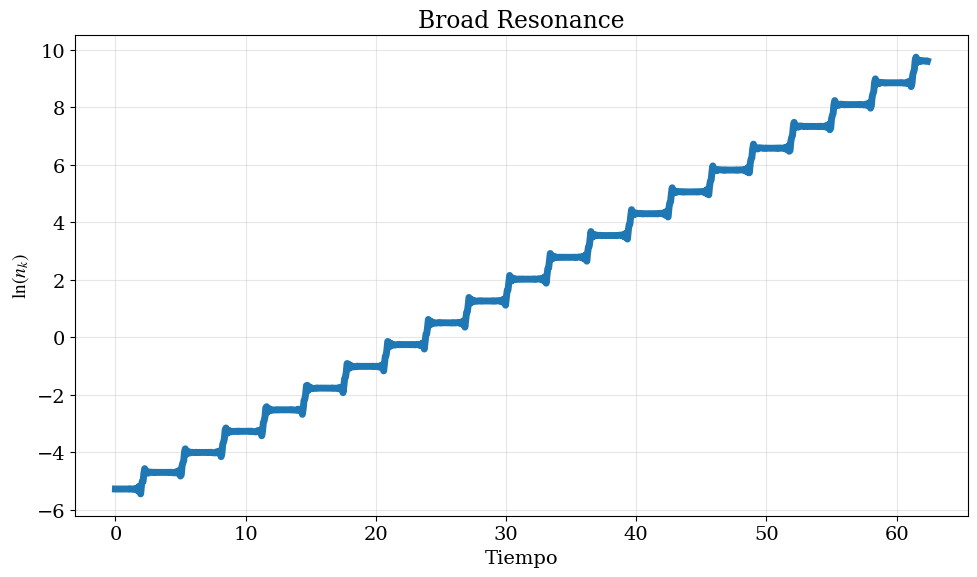
\includegraphics[width = \linewidth]{Imagenes/Nahue/n_broad.png}
        \caption{broad resonance: $q = 5050$ y $k = 6.4686076615463275$}
        \label{fig:n_broad}
    \end{subfigure}
    \caption{evolución del número de partículas en el tiempo.}
\end{figure}

En este mismo código podemos armarnos un espectro de potencias que lo que hace es calcular el valor cuadrado de $\chi_k$ y podemos ver que este espectro para $q = 5050$ crece como $k^3$ por tanto para poder ver el espectro lineal y comparar si existe un pico para las frecuencias dónde tenemos una banda de resonancia. Ésto se puede ver en la figura \ref{fig:Pchi_lphi4} dónde vemos que es muy ruidoso el espectro de potencias y se puede deber a la resolución que se le asigna al espectro. También, en la figura \ref{fig:Pchi_lphi4_vart} podemos ver cómo evoluciona este espectro en el tiempo en el cual podemos ver que a medida que aumenta el tiempo el pico crece y el ruido se homogeniza.

\begin{figure}[H]
    \centering
    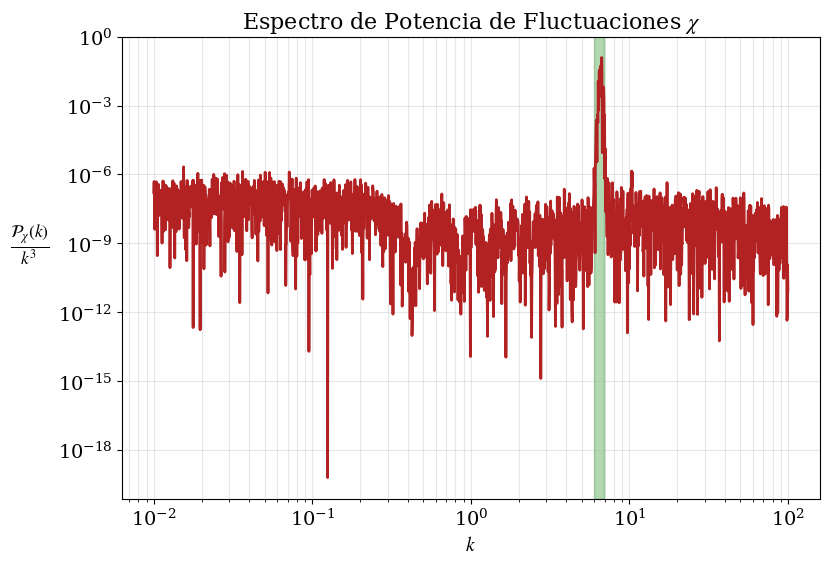
\includegraphics[width = \linewidth]{Imagenes/Nahue/Pchi.png}
    \caption{espectro de potencias lineal para las fluctuaciones del campo hijo.}
    \label{fig:Pchi_lphi4}
\end{figure}

\begin{figure}[H]
    \centering
    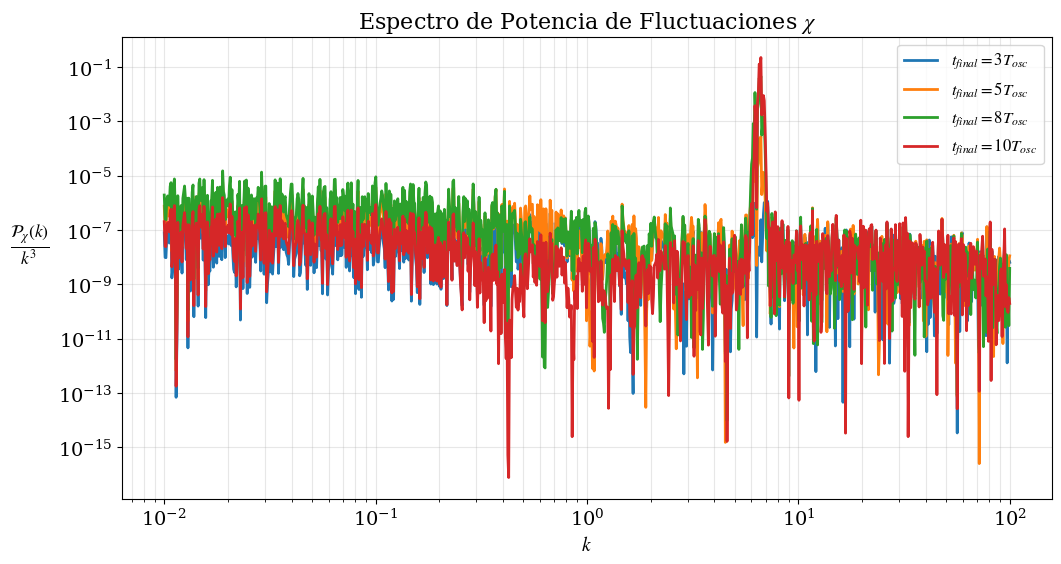
\includegraphics[width = \linewidth]{Imagenes/Nahue/Pchi_vart.png}
    \caption{espectro de potencias lineal para las fluctuaciones del campo hijo para distintos tiempos.}
    \label{fig:Pchi_lphi4_vart}
\end{figure}

Finalmente, una vez que armamos el espectro de potencias, podemos armar el espectro de ondas gravitacionales que es el que se puede observar en la figura \ref{fig:GW_lphi4}, en la misma podemos ver que efectivamente en la banda de resonancia de Floquet se observa una amplificación en la densidad de energía, pero el label nos indica que lo que graficamos es $\Omega_{GW}$ aunque ésto es incorrecto ya que nos está dando mayor que $1$ lo que no tiene sentido físico, además le falta dividir por la densidad de energía crítica, pero sí debería decir $\displaystyle \frac{d \rho_{GW}}{d \ln k}$.

\begin{figure}[H]
    \centering
    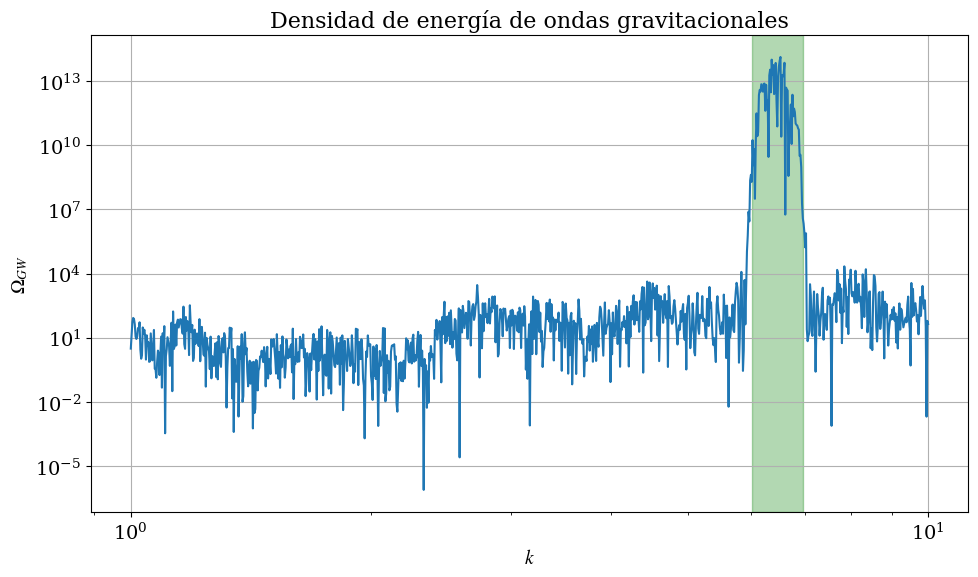
\includegraphics[width = \linewidth]{Imagenes/Nahue/lphi4_GW.png}
    \caption{distribución en $k$ para la densidad de energía de ondas.}
    \label{fig:GW_lphi4}
\end{figure}

El espectro de ondas gravitacionales lo podemos calcular a partir de las fluctuaciones del campo hijo a partir de la expresión derivada previamente que es de la forma

\begin{equation}
    \frac{d \rho_{\text{GW}}}{d \ln k} = \frac{k^3}{16 \pi^4 m_p^2 a^4} \int p^6 \sin^5 \theta ~ \left[ \left| I_{(c)} (k, p, \theta, \tau)  \right|^2 + \left| I_{(s)} (k, p, \theta, \tau)  \right|^2 \right] ~ dp ~ d\theta
\end{equation}

\noindent
dónde $I_{(s)}$ e $I_{(c)}$ están definidas a partir de

$$I_{(c)} (k, p, \theta, \tau) = \int_{\tau_{i}}^\tau  \frac{\cos (k\tau^\prime)}{a \left( \tau^\prime \right)} ~ \chi^{(c)}_{p} (\tau^\prime) ~ \chi_{k - p}^{(c)} (\tau^\prime) ~ d\tau^\prime$$

$$I_{(s)} (k, p, \theta, \tau) = \int_{\tau_{i}}^\tau  \frac{\sin (k\tau^\prime)}{a \left( \tau^\prime \right)} ~ \chi^{(c)}_{p} (\tau^\prime) ~ \chi_{k - p}^{(c)} (\tau^\prime) ~ d\tau^\prime$$

\noindent
y los $\chi_k^{(c)}$ es la dinámica del campo hijo que conseguimos previamente.

\subsubsection{Con expansión}

Si agregamos expansión a lo que hicimos anteriormente, podemos graficar cómo es el background en la figura \ref{fig:lphi4_background} dónde vemos cómo evoluciona el inflatón (\ref{fig:inf_lphi4}), el parámetro de escala (\ref{fig:a_lphi4}) y el de Hubble (\ref{fig:H_lphi4}) en el tiempo. Podemos ver que efectivamente el inflatón decae en el tiempo por consecuencia de la expansión del universo, mientras que el universo se expande como se espera y el parámetro de Hubble decae abruptamente como conseciencia de la caída en la velocidad de expansión del universo que ocurre por el decaimiento del inflatón.

\begin{figure}[H]
    \centering
    \begin{subfigure}[t]{0.6\linewidth}
        \centering
        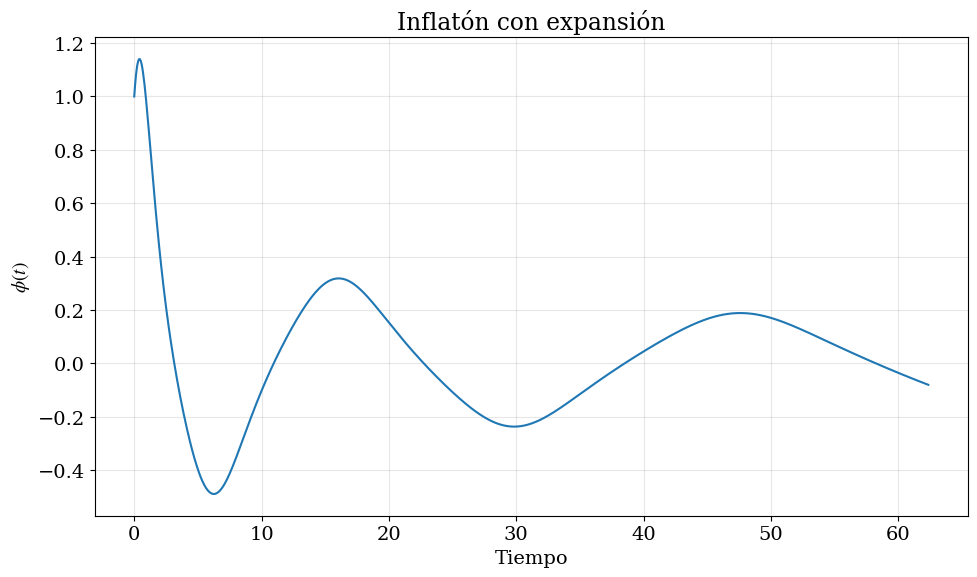
\includegraphics[width = \linewidth]{Imagenes/Nahue/inflaton_lphi4.png}
        \caption{evolución del inflatón en el tiempo}
        \label{fig:inf_lphi4}
    \end{subfigure}
    \begin{subfigure}[b]{0.45\linewidth}
        \centering
        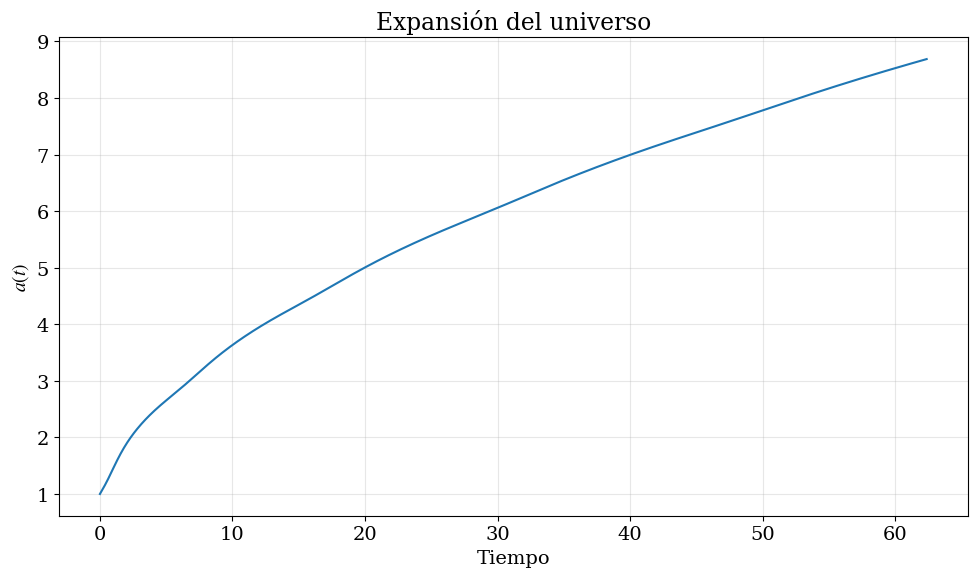
\includegraphics[width = \linewidth]{Imagenes/Nahue/a_lphi4.png}
        \caption{evolución del parámetro de escala en el tiempo}
        \label{fig:a_lphi4}
    \end{subfigure}
    \begin{subfigure}[b]{0.45\linewidth}
        \centering
        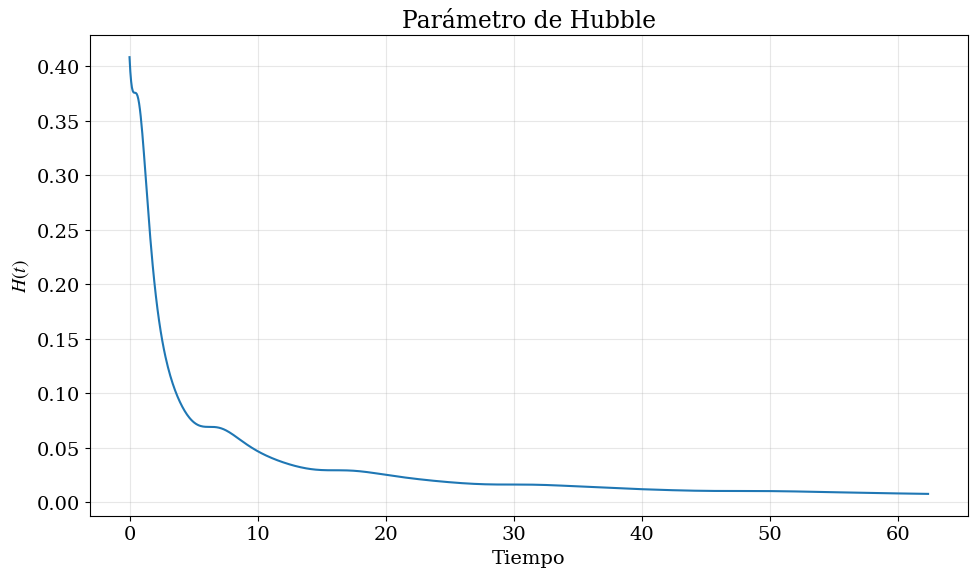
\includegraphics[width = \linewidth]{Imagenes/Nahue/H_lphi4.png}
        \caption{evolución del parámetro de Hubble en el tiempo}
        \label{fig:H_lphi4}
    \end{subfigure}
    \caption{evolución del background para el modelo $\lambda \phi^4$.}
    \label{fig:lphi4_background}
\end{figure}

Luego, se reutilizaron los valores de $k$ y $q$ para formar la narrow y broad resonance volviendo a obtener gráficos similares a los que obtuvimos sin expansión y por tanto consistentes a lo esperado. Éstos gráficos con las dinámicas se pueden observar en las figuras \ref{fig:lphi4_narrow_exp} y \ref{fig:lphi4_broad_exp}. Además, en las figuras \ref{fig:n_narrow_exp} y \ref{fig:n_broad_exp} podemos ver cómo es la evolución del número de ocupación en el tiempo, en estas figuras podemos notar un comportamiento que decae como consecuencia de la expansión del universo mientras podemos notar también un comportamiento no esperado si comparamos con una resonancia estocástica.

\begin{figure}[H]
    \begin{subfigure}[t]{0.5\linewidth}
        \centering
        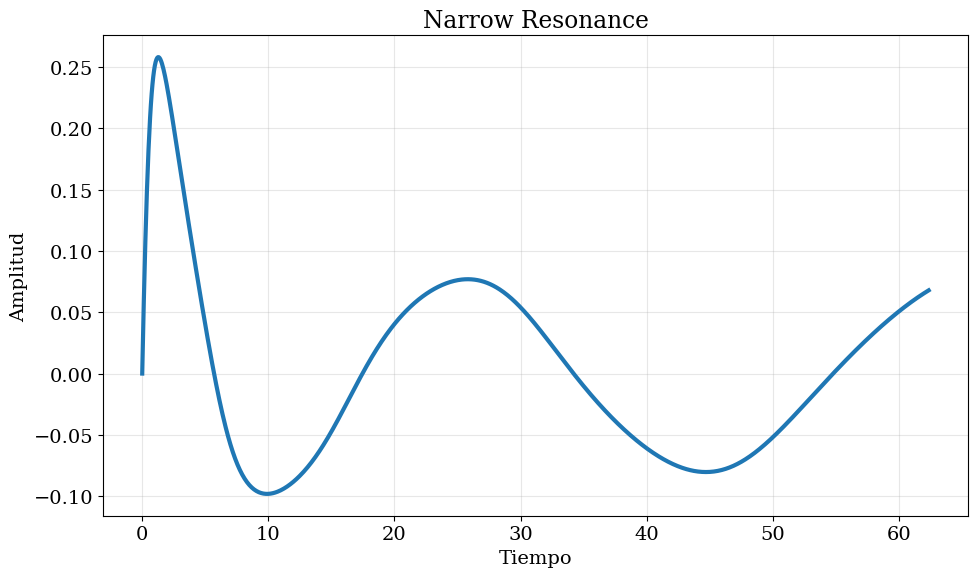
\includegraphics[width = \linewidth]{Imagenes/Nahue/lphi4_narrow_exp.png}
        \caption{narrow resonance: $q = 0.5$ y $k = 0.8277856966198477$}
        \label{fig:lphi4_narrow_exp}
    \end{subfigure}
    \begin{subfigure}[t]{0.5\linewidth}
        \centering
        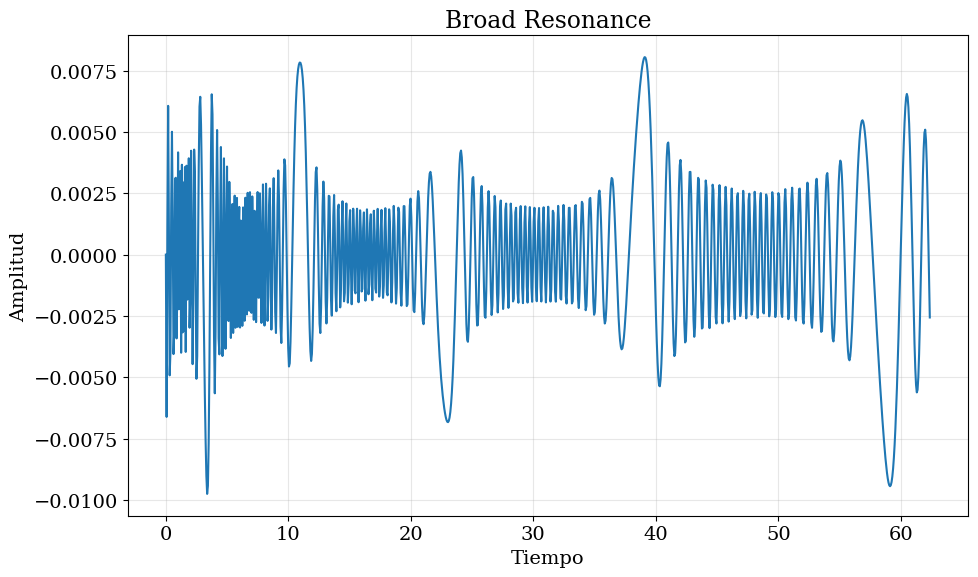
\includegraphics[width = \linewidth]{Imagenes/Nahue/lphi4_broad_exp.png}
        \caption{broad resonance: $q = 5050$ y $k = 6.4686076615463275$}
        \label{fig:lphi4_broad_exp}
    \end{subfigure}
    \caption{evolución de las resonancias en el tiempo.}
\end{figure}

\begin{figure}[H]
    \begin{subfigure}[t]{0.5\linewidth}
        \centering
        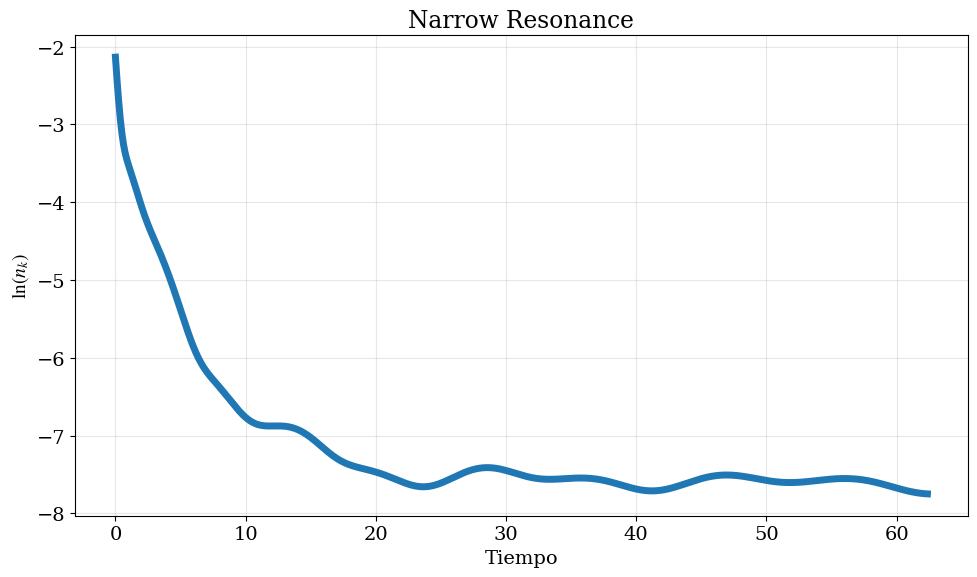
\includegraphics[width = \linewidth]{Imagenes/Nahue/n_narrow_exp.png}
        \caption{narrow resonance: $q = 0.5$ y $k = 0.8277856966198477$}
        \label{fig:n_narrow_exp}
    \end{subfigure}
    \begin{subfigure}[t]{0.5\linewidth}
        \centering
        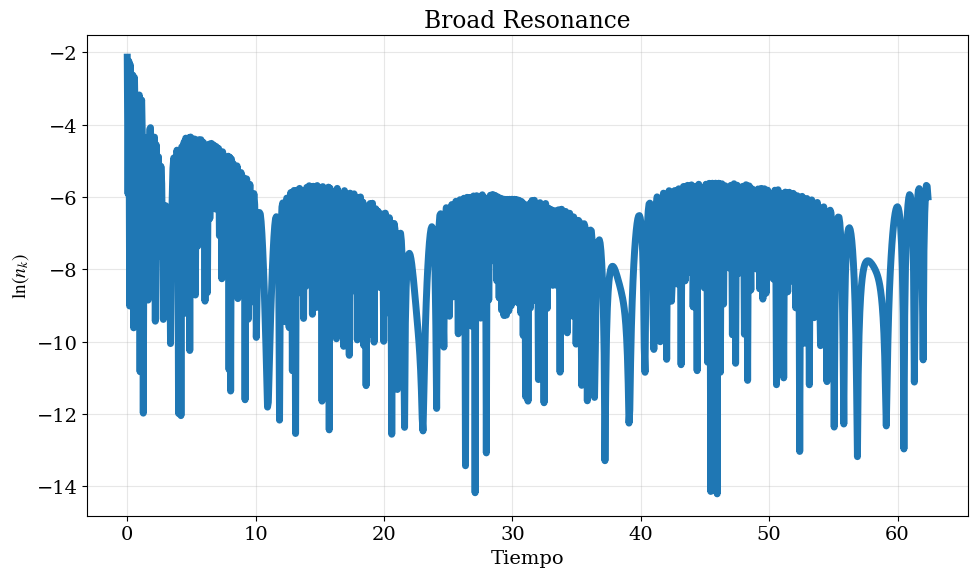
\includegraphics[width = \linewidth]{Imagenes/Nahue/n_broad_exp.png}
        \caption{broad resonance: $q = 5050$ y $k = 6.4686076615463275$}
        \label{fig:n_broad_exp}
    \end{subfigure}
    \caption{evolución del número de partículas en el tiempo.}
\end{figure}

Una vez estudiada la dinámica y el número de partículas para cada tipo de resonancia, podemos armar el espectro de potencias para el campo con expansión para $q = 5050$ y verlo en la figura \ref{fig:Pchi_lphi4_exp} y variando en el tiempo en \ref{fig:Pchi_lphi4_vart_exp}, dónde comparado al espectro sin expansión podemos notar que no existe el pico de resonancia, ésto dá a pensar que hay un error en el código pero aún no logro encontrarlo.

\begin{figure}[H]
    \centering
    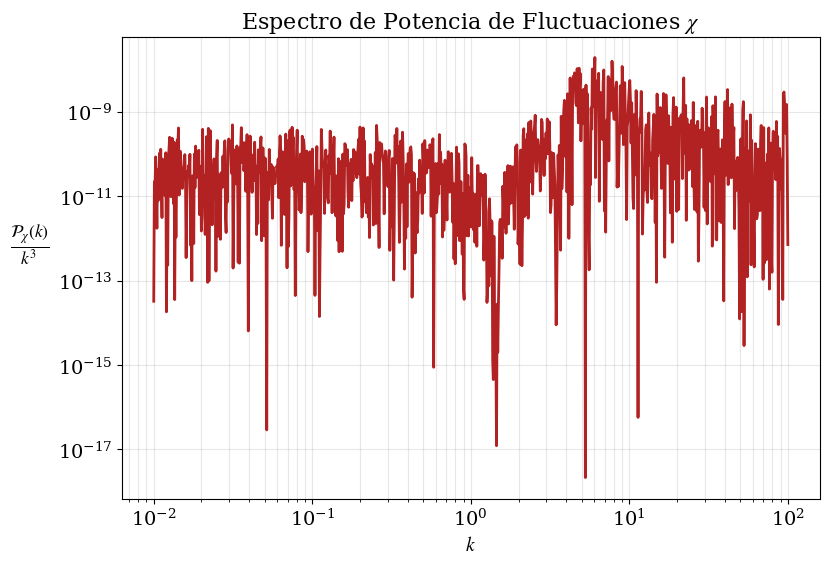
\includegraphics[width = \linewidth]{Imagenes/Nahue/Pchi_exp.png}
    \caption{espectro de potencias lineal para las fluctuaciones del campo hijo.}
    \label{fig:Pchi_lphi4_exp}
\end{figure}

\begin{figure}[H]
    \centering
    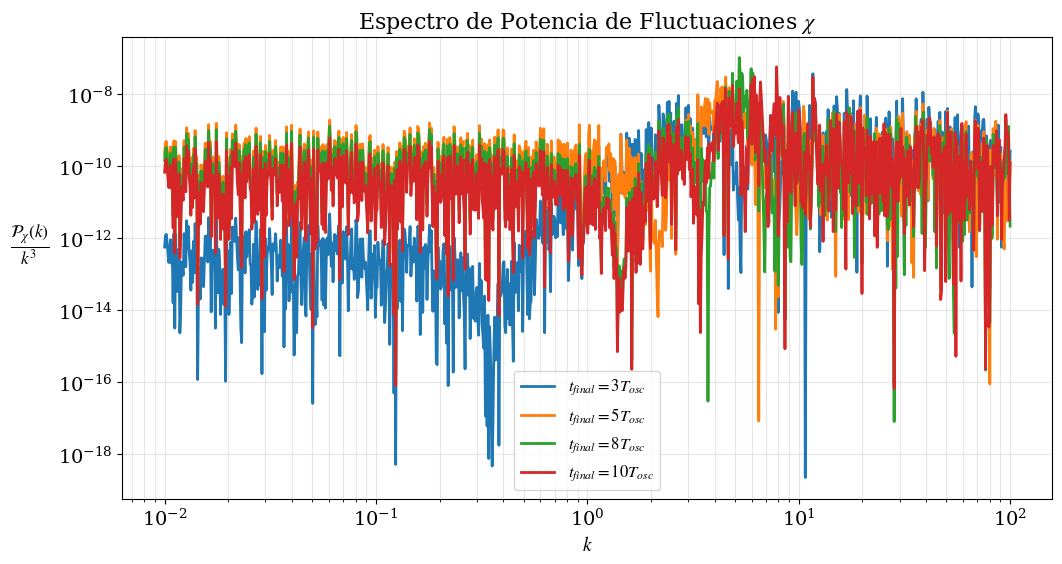
\includegraphics[width = \linewidth]{Imagenes/Nahue/Pchi_vart_exp.png}
    \caption{espectro de potencias lineal para las fluctuaciones del campo hijo para distintos tiempos.}
    \label{fig:Pchi_lphi4_vart_exp}
\end{figure}

\subsubsection{Reescaleo del espectro de potencia de GWs hoy}

Con CosmoLattice, podemos obtener el espectro de potencia de las ondas gravitacionales en términos del número de onda adimensionalizado $\tilde{k}$ y lo que buscamos poder conseguir es el espectro de potencias en términos de la frecuencia física que podemos medir hoy. Para poder reescalar el espectro a hoy debemos tener en cuenta que en las simulaciones de CosmoLattice a partir de un cierto tiempo $t_*$ los espectros de las ondas se saturan, haciendo que no se produzcan más ondas durante Reheating, eso mismo implica que desde este tiempo hasta un tiempo $t_{reh}$ para el cual termina Reheating vale:

\begin{equation}
    \Omega_{GW} \left( k, t_{reh} \right) = \Omega_{GW} \left( k, t_* \right)
\end{equation}

Por otro lado, para ver cómo se reescala el espectro cuando estamos en las eras posteriores debemos recordar que $\Omega = \rho / \rho_C$, para la densidad de las ondas gravitacionales, sabemos que siempre va como $\rho_{GW} \propto a^4$ mientras que la densidad de energía crítica va como $\rho \propto a^4$ cuando estamos en radiación y va como $\rho \propto a^3$ cuando estamos en materia, lo que implica que el espectro de ondas se reescala de la siguiente forma:

\begin{equation*}
    \begin{split}
        \Omega_{GW} \left( k, t_0 \right) &= \frac{\rho_{GW} \left( t_0 \right)}{\rho_C \left( t_0 \right)}\\
        &= \frac{(a_{eq}/a_0)^4 \rho_{GW} \left( k, t_{eq} \right)}{(a_{eq}/a_0)^3 \rho_C \left( k, t_{eq} \right)}\\
        &= \frac{a_{eq}}{a_0} \frac{\rho_{GW} \left( k, t_{eq} \right)}{\rho_C \left( k, t_{eq} \right)}\\
        &= \frac{a_{eq}}{a_0} \frac{(a_{reh}/a_{eq})^4 \rho_{GW} \left( k, t_{reh} \right)}{(a_{reh}/a_{eq})^4 \rho_C \left( k, t_{reh} \right)}\\
        &= \frac{a_{eq}}{a_0} \frac{\rho_{GW} \left( k, t_{reh} \right)}{\rho_C \left( k, t_{reh} \right)}\\
        &= \frac{a_{eq}}{a_0} \Omega_{GW} \left( k, t_{reh} \right)
    \end{split}
\end{equation*}

\begin{equation}
    \Omega_{GW} \left( k, t_0 \right) = \frac{a_{eq}}{a_0} \Omega_{GW} \left( k, t_{*} \right)
\end{equation}

\noindent
finalmente debemos saber que la relación $a_{eq}/a_0 = 1/3000$ y con ello podemos obtener el espectro de potencias reescalado a tiempo hoy. 

Finalmente, nos falta escribir el espectro de potencias de las ondas en términos de la frecuencia física hoy que lo podemos hacer sabiendo que la relación entre $\tilde{k}$ y $f$ está dada por:

\begin{equation}
    f = \frac{a_i}{a_0} \frac{k}{2\pi} = \frac{a_{reh}}{a_0} \frac{\omega_* \tilde{k}}{2\pi}
\end{equation}

\noindent
y podemos usar que $a \propto 1/T$

\begin{equation}
    f = \frac{T_{0}}{T_{reh}} \frac{\omega_* \tilde{k}}{2 \pi}
\end{equation}